%-------------------------------------------------------------------------------
% DOCUMENT CLASS & PACKAGES
%-------------------------------------------------------------------------------
\documentclass[12pt,twoside, openright]{memoir}
\usepackage{graphicx, wrapfig, subcaption, setspace, booktabs, amsmath, float, lettrine}
\usepackage[a4paper]{geometry}
\usepackage{fancyhdr, tabto, emptypage, lastpage, pdfpages, appendix, epigraph}
\usepackage{booktabs, multirow, siunitx, tabularx}
\usepackage[protrusion=true, expansion=true]{microtype}
\usepackage[utf8]{inputenc}
\usepackage[T1]{fontenc}
\usepackage[francais]{babel}
\usepackage{algorithm}
\usepackage[noend]{algpseudocode}
\makeatletter
\def\BState{\State\hskip-\ALG@thistlm}
\makeatother
\mathchardef\hyphenmathcode=\mathcode`\-
\usepackage{breqn, url}
\usepackage{listings, enumitem, array, minted}

\frenchbsetup{StandardItemLabels=true}
\renewcommand{\labelitemi}{$\bullet$}

\newcolumntype{P}[1]{>{\centering\arraybackslash}p{#1}}

\usepackage{color, colortbl, xcolor}
\definecolor{codegreen}{rgb}{0,0.6,0}
\definecolor{codegray}{rgb}{0.5,0.5,0.5}
\definecolor{codepurple}{rgb}{0.58,0,0.82}
\definecolor{backcolour}{rgb}{0.98,0.98,0.98}

\renewcommand{\ttdefault}{fvm}
\makeatletter\renewcommand*{\@biblabel}[1]{\hfill#1.}\makeatother
\newcommand{\HRule}[1]{\rule{\linewidth}{#1}}
\newcolumntype{L}[1]{>{\raggedright\let\newline\\\arraybackslash\hspace{0pt}}m{#1}}
\newcolumntype{C}[1]{>{\centering\let\newline\\\arraybackslash\hspace{0pt}}m{#1}}
\newcommand{\courrier}[1]{{\fontfamily{qcr}\selectfont {#1}}}
\setcounter{tocdepth}{5}
\setcounter{secnumdepth}{5}

\usepackage[nopostdot,style=super,nonumberlist,toc,section=chapter]{glossaries}
\newglossaryentry{cr}{name={CR},description={CheiRank}}
\newglossaryentry{pr}{name={PR},description={PageRank}}
\newglossaryentry{tr}{name={TR},description={TrustRank}}
\newglossaryentry{csv}{name={CSV},description={Comma Separated Values}}
\newglossaryentry{sql}{name={SQL},description={Structured Query Language}}
\newglossaryentry{url}{name={URL},description={Uniform Ressource Locator}}
\newglossaryentry{seo}{name={SEO},description={Search Engine Optimization}}
\newglossaryentry{apoc}{name={APOC},description={Awesome Procedures On Cypher}}
\newglossaryentry{hits}{name={HITS},description={Hyperlink-Induced Topic Search}}
\newglossaryentry{html}{name={HTML},description={HyperText Markup Language}}
\newglossaryentry{http}{name={HTTP},description={HyperText Transfer Protocol}}
\newglossaryentry{json}{name={JSON},description={JavaScript Object Notation}}
\newglossaryentry{ascii}{name={ASCII},description={American Standard Code for Info Interchange}}
\newglossaryentry{arpanet}{name={ARPANET},description={Advanced Research Projects Agency Network}}
\makenoidxglossaries

%-------------------------------------------------------------------------------
% TITLES
%-------------------------------------------------------------------------------
\definecolor{partred}{rgb}{.341,.094,.271}
\definecolor{chapterred}{rgb}{.565,.047,.243}
\definecolor{sectionred}{rgb}{.780,.000,.224}
\definecolor{subsectionorange}{rgb}{1.00,.341,.200}
\makechapterstyle{mym}{%
	\renewcommand\chapnamefont{\normalfont\Huge\bfseries\color{chapterred}}%
	\renewcommand\chaptitlefont{\normalfont\Huge\bfseries\color{chapterred}}%
	\renewcommand\printchapternonum{}%
	\renewcommand\printchaptertitle[1]{\chaptitlefont ##1}%
}
\chapterstyle{mym}
\usepackage{titlesec}
\titleformat*{\section}{\normalfont\Large\bfseries\color{sectionred}}
\titleformat*{\subsection}{\normalfont\large\bfseries\color{subsectionorange}}

\let\oldafterpartskip\afterpartskip % save definition
\newcommand\partepigraph[3][100pt]{
	\renewcommand{\afterpartskip}{%
		\vskip#1
		{\color{black}\epigraph{#2}{#3}}
		\vfil}
}
\newcommand\removeepigraph{%
	\let\afterpartskip\oldafterpartskip} % restore definition

%-------------------------------------------------------------------------------
% HEADER & FOOTER
%-------------------------------------------------------------------------------
\pagestyle{fancy}
\fancyhf{}
\setlength\headheight{15pt}
\renewcommand{\chaptermark}[1]{\markboth{\thechapter.\ #1}{}}
\fancyhead[LO]{\itshape{Les algorithmes du Web}}
\fancyhead[RE]{\itshape{\leftmark}}
\fancyfoot[C]{\bfseries\thepage}

\fancypagestyle{plain}{% %
	\fancyhf{}%
	\fancyfoot[C]{\bfseries\thepage}
	\renewcommand{\headrulewidth}{0pt}%
}

\renewcommand\cftappendixname{\appendixname~}

\makeatletter
\setlength\@tempdima       {\paperwidth}
\addtolength\@tempdima     {-\textwidth}
\setlength\oddsidemargin   {.5\@tempdima}
\addtolength\oddsidemargin {-1in}
\setlength\marginparwidth  {.5\@tempdima}
\addtolength\marginparwidth{-\marginparsep}
\addtolength\marginparwidth{-0.8in} % don't know why this isn't .4
\setlength\evensidemargin\oddsidemargin
\makeatother

\begin{document}
	\renewcommand{\appendixtocname}{Annexes}
	\renewcommand{\appendixpagename}{Annexes}
	\renewcommand{\contentsname}{Table des matières}
	\renewcommand{\bibname}{Bibliographie}
	
	%-------------------------------------------------------------------------------
	% TITLE PAGE
	%-------------------------------------------------------------------------------
	
\includepdf[page=1, scale=.95]{pdf/firstpage.pdf}
	\cleardoublepage
	
	%-------------------------------------------------------------------------------
	% ACKNOWLEDGMENTS
	%-------------------------------------------------------------------------------
	\chapter*{Remerciements}
	\addcontentsline{toc}{chapter}{Remerciements}
	Alors que je m'apprête à déposer ce mémoire sur les serveurs de Hepia, le rendant public pour les années à venir, je suis à même de constater que sa réalisation n'aurait pu être effectuée comme telle sans l'aide de quelques personnes que je ne vais surtout pas manquer de remercier.
	\vskip.3cm
	Je souhaiterais commencer par remercier mon professeur encadrant Mr. Orestis Malaspinas pour son aide précieuse tout au long de ce travail. Il a su me fournir des conseils justes relatifs à mes points faibles que j'ai pu par la suite corriger, du moins je l'espère.
	\vskip.3cm
	J'aimerais également remercier mes camarades de bureau Kevin, Gabriel, Alexandre pour leur soutien constant durant ces trois dernières années. Ils ont su me pousser pour améliorer mes performances et mon sérieux dans mon travail. Merci les gars.
	\vskip.3cm
	Un merci maintenant addressé aux deux personnes qui ont relu ce mémoire, sans qui  de nombreuses fautes de syntaxe seraient sans doute toujours présentes.\par
	Merci à toi Basile, tout juste bachelier et plein de bonne volonté. Tu as toujours été là pour moi. Je comprends que c'était un travail difficile de relire cette thèse pour me corriger, mais tu as persévéré et ton aide m'a été bien plus que précieuse. Merci mon poulet !\par
	Quant à toi, Sophie, ma chère tante plus connue sous le surnom de "Didi", merci pour tes conseils, ta patience, ta persévérance et ta rigueur d'esprit qui m'ont beaucoup aidé dans la rédaction de cette thèse, mais pas que !
	\vskip.3cm
	Enfin, je remercie ma mère pour m'avoir toujours guidé dans mes choix, parfois simples, parfois difficiles. Tu m'as sans relâche remis dans le droit chemin lorsque je commençais à chavirer et tes conseils, parfois si évidents, m'ont été d'un grand secours. Merci pour tout Maman.
	\cleardoublepage
	
	%-------------------------------------------------------------------------------
	% TABLE OF CONTENTS
	%-------------------------------------------------------------------------------
	\tableofcontents*
	\cleardoublepage
	
	%-------------------------------------------------------------------------------
	% WORK TO DO
	%-------------------------------------------------------------------------------
	
\includepdf[pagecommand={\addcontentsline{toc}{chapter}{Enoncé du sujet} \thispagestyle{empty}}]{pdf/ITI_IN_enonce_diplome_Ollquist_Malaspinas_2019.pdf}
	\cleardoublepage
	
	%-------------------------------------------------------------------------------
	% ABSTRACT
	%-------------------------------------------------------------------------------
	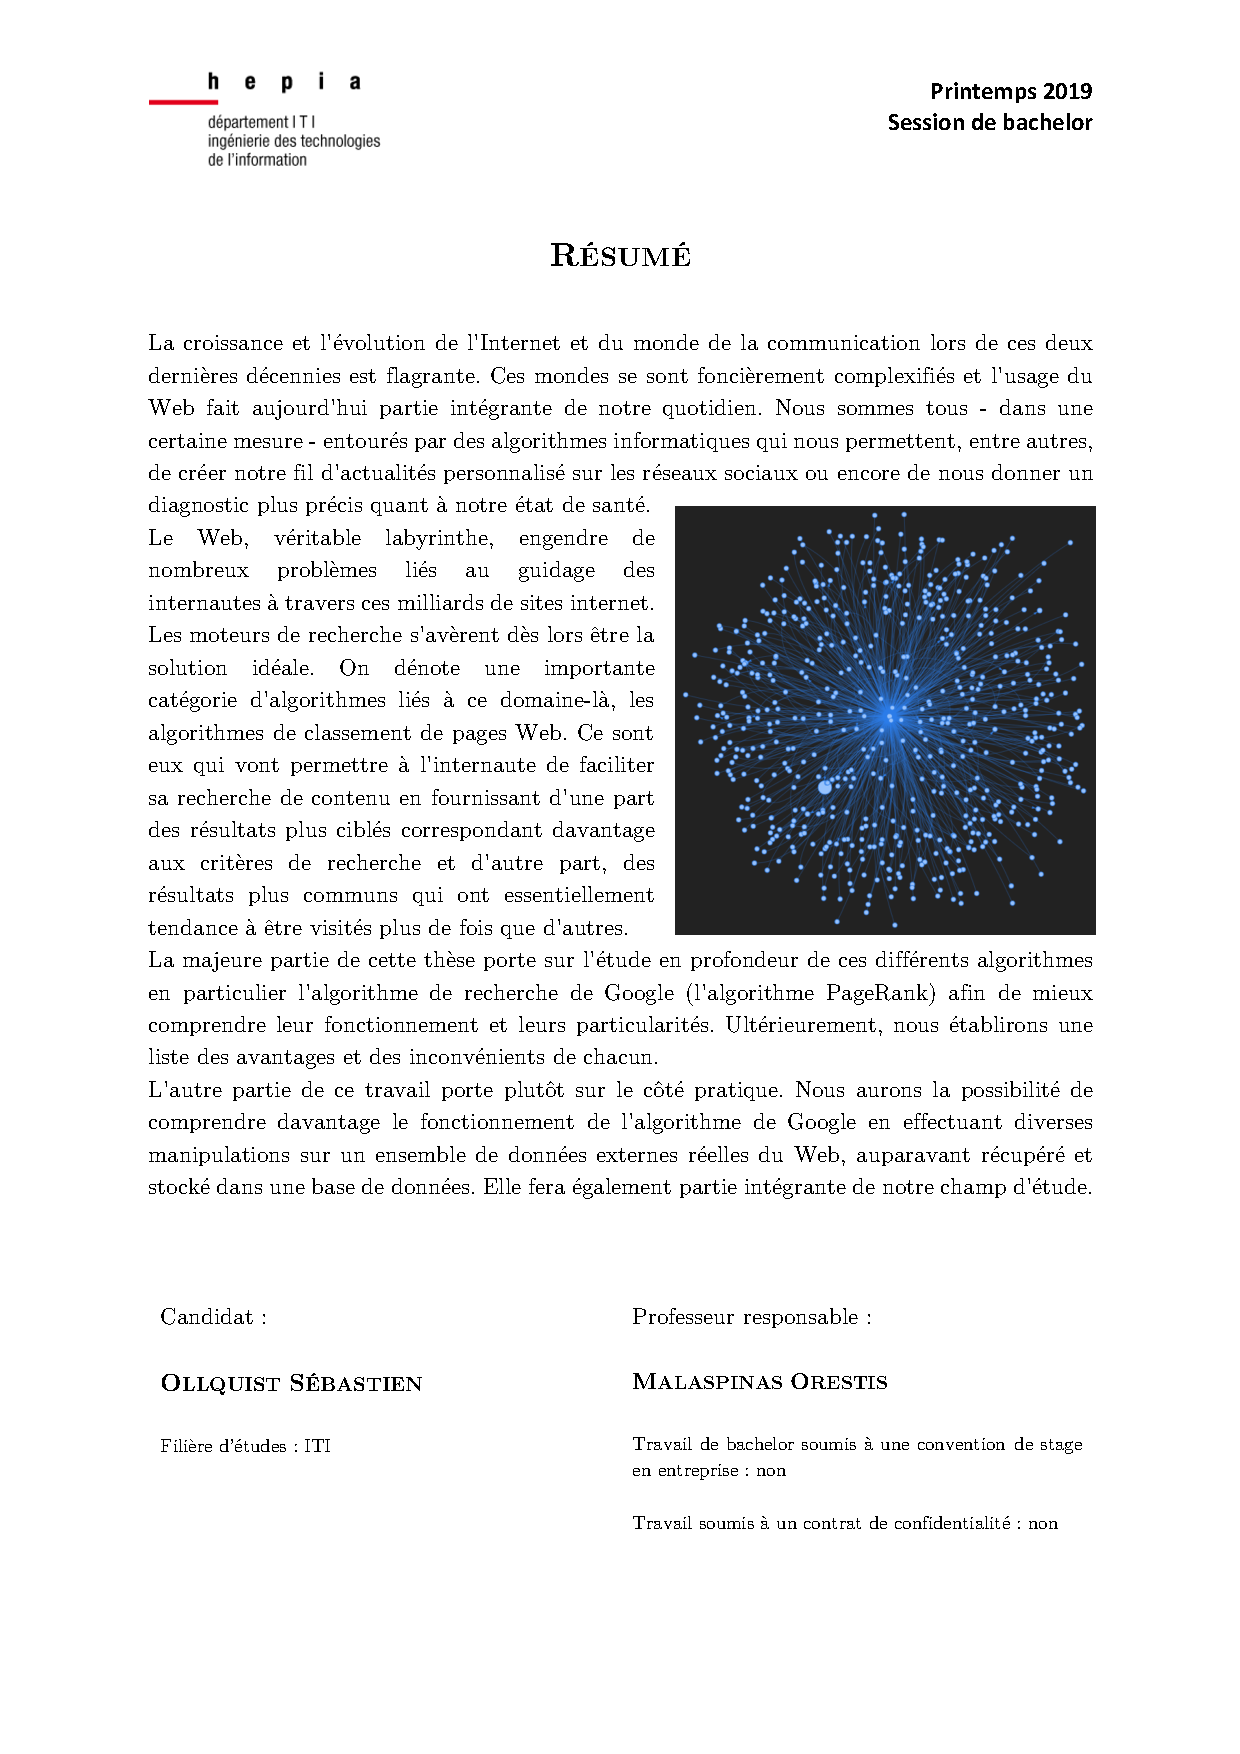
\includepdf[pagecommand={\addcontentsline{toc}{chapter}{Résumé} \thispagestyle{empty}}]{pdf/resume.pdf}
	\cleardoublepage
	
	%-------------------------------------------------------------------------------
	% TABLE OF FIGURES
	%-------------------------------------------------------------------------------
	\listoffigures
	\cleardoublepage
	
	%-------------------------------------------------------------------------------
	% GLOSSARY
	%-------------------------------------------------------------------------------
	\printnoidxglossary[title={Liste des acronymes}]
	
	%-------------------------------------------------------------------------------
	% BODY
	%-------------------------------------------------------------------------------
	\chapter*{Introduction}
	\markboth{Introduction}{}
	\addcontentsline{toc}{chapter}{Introduction}
	\lettrine[lraise=0.1, nindent=0em]{D}{epuis} de nombreuses années, l'Internet et plus particulièrement le Web se sont métamorphosés. On recense toujours plus de sites, de données et de machines accessibles aux internautes. Lors de la création du Web, le problème majeur était la possibilité pour un internaute de retrouver son chemin parmi des millions voire des milliards de sites internet. La création d'un moteur de recherche, pour guider les internautes à travers ce grand labyrinthe était alors inévitable. La firme Google possède depuis plus de vingt ans le quasi monopole du secteur des moteurs de recherche ce qui fait d'elle, l'archétype de la réussite moderne.
	\vskip.5cm
	Aujourd'hui, les algorithmes informatiques ont envahi notre vie quotidienne, on les retrouve en effet dans bon nombre de nos habitudes. Pourtant, malgré leur omniprésence et leur importance dans notre vie, ils restent pour la plupart relativement obscurs au grand public. Ce sont eux qui permettent la construction de notre fil d'actualités sur les réseaux sociaux, l'accélération des transactions boursières ou encore l'orientation des internautes vers des produits spécifiques suite à leur achat sur internet. Toutes ces activités sont aujourd'hui partie intégrante de notre quotidien.
	\vskip.5cm
	On note une autre catégorie d'algorithmes tous aussi importants, visant à classer des sites internet en leur donnant une certaine quote de popularité. Les moteurs de recherche se servent pour la plupart de ces algorithmes de classement. Ils ont comme principal objectif de donner des scores à chacune des pages. Certains de ces scores se basent sur des critères concrets. Google possède son propre algorithme de ranking: le PageRank (abrévié \gls{pr}). C'est cet algorithme, régissant le classement des pages Web sur internet, qui sera le principal objet de notre étude.
	\vskip.5cm
	Il existe également des alternatives au \gls{pr}, utilisées notamment par le reste des moteurs de recherche présents sur le Web. Ce sont entre autres, le \gls{hits} pour Yahoo ou le \gls{cr}, plus développé que le \gls{pr}. Ces alternatives se distinguent du \gls{pr} en possédant notamment un certain nombre de critères supplémentaires.
	\vskip.5cm
	Depuis mes débuts dans l'informatique, je ne cesse de m'intéresser au monde des sciences et de la technologie. L'une de mes principales sources de motivation est le simple fait de pouvoir créer librement des programmes qui me sont utiles en mettant à profit de nouvelles technologies. J'ai tout de suite saisi l'opportunité de réaliser le travail de mon choix en associant mathématiques et informatique. Le sujet du \gls{pr} m'est de suite venu à l'esprit. Je souhaitais en apprendre davantage sur l'une des faces cachées de Google et ce travail était une opportunité à ne pas manquer.
	\vskip.5cm
	L'objectif principal de ce mémoire est de comprendre dans un premier temps comment fonctionnent ces algorithmes de classement et sur quels critères ils se basent. Dans un second temps, de les comparer afin de déterminer, in fine, lequel est le plus fiable.
	\vskip.5cm
	Le premier chapitre a pour objectif d'initier le lecteur au monde du Web. Nous retraçerons d'abord l'historique du Web, de ses débuts fulgurants à son influence mondiale actuelle. Nous chercherons ensuite à en donner une définition plus précise. Puis nous introduirons la notion de référencement.\par
	Le deuxième chapitre a pour but de comprendre plus en profondeur la finalité du \gls{pr} et son fonctionnement au sein de l'Internet. Nous favoriserons une approche plus mathématique en détaillant quelques points de vue théoriques. Puis nous décrirons étape par étape comment se comporte l'algorithme. Nous donnerons ensuite un exemple d'application et nous ferons varier les différents paramètres qu'utilise l'algorithme afin de noter l'influence qu'ils peuvent avoir sur l'agissement de celui-ci.\par
	Dans le chapitre 3, nous proposerons quelques alternatives au \gls{pr} en faisant une liste exhaustive des avantages et des inconvénients qu'ils peuvent avoir. Nous proposerons également une implémentation de chacune d'entre elles en Python.\par
	Nous nous familiariserons avec l'outil Neo4j au cours du chapitre 4 pour créer, manipuler et afficher des graphes (parfois complexes). Nous créerons d'abord des graphes simples manuellement puis nous importerons des données externes réelles beaucoup plus imposantes afin d'y appliquer l'algorithme \gls{pr}.\par
	Pour finir, nous appliquerons dans le chapitre 5 l'algorithme \gls{pr} à un graphe plus conséquent et nous effectuerons une série de tests accompagnée d'une visualisation minimale pour mieux saisir la situation.
	
	%-------------------------------------------------------------------------------
	% PART I : THEORY	%-------------------------------------------------------------------------------
	\partepigraph{\textit{« Qui maîtrise l'Internet, maîtrise le Monde. »}}{-- Christophe Bonnefont}
	{\color{partred}\part{Les algorithmes du Web}}
	\removeepigraph
	
	%-------------------------------------------------------------------------------
	% WORLD WIDE WEB	%-------------------------------------------------------------------------------
	\chapter{La naissance du Web}
	\lettrine[lraise=0.1, nindent=0em]{A}{vant} de rentrer dans les particularités du Web, il semble nécessaire de retracer son historique pour mieux décrire ses principaux composants et mieux évaluer la quantité de données qu'il contient.
	\section{Création du World Wide Web}
	Vers la fin des années 1950 aux Etats-Unis, les laboratoires Bell créent leur premier modem permettant d'envoyer des données informatiques sur une ligne téléphonique. L'idée d'un premier réseau interconnecté d'ordinateurs est alors évoquée.\par
	En 1967 a lieu la première conférence \gls{arpanet}, point de départ de l'Internet actuel. Alors, seuls 4 ordinateurs dans le monde servent de serveurs \footnote{Cette donnée et les suivantes recensées dans ce chapitre sont tirées du site internet de l'Université de Rennes. Voir: \url{https://www.sites.univ-rennes2.fr/urfist/internet_chiffres}}.\par
	C'est au cours des années 1980 qu'apparaît le Web tel que nous le connaissons aujourd'hui. Les premiers ordinateurs apparaissent à destination du "grand public" et la révolution informatique est lancée.\par
	En 1984, le CERN (Centre Européen de Recherche Nucléaire) rejoint Internet. Sept ans plus tard, il crée le "World Wide Web". Le nombre d'ordinateurs connectés est alors d'environ 617'000.\par
	Conséquence de cette explosion, la nécessaire organisation du Web voit l'émergence des moteurs de recherche. Créée en 1998, Google est aujourd'hui une référence dans le domaine.\newpage
	\begin{table}[h]
		\centering
		\begin{tabularx}{14cm}{ cccc }
			\toprule[1.5pt]
			\textbf{Fait} & \textbf{En 1998} & \textbf{En 2013} & \textbf{En 2018}\\
			\hline
			Nombre de pages Web indexées & $26$ M & $60'000$ Mds & $130'000$ Mds \\
			\hline
			Nombre de requêtes par mois & $10'000$ & $3,3$ Mds & $168$ Mds \\
			\hline
			Nombre d'employés & $3$ & $44'777$ & $98'771$ \\
			\bottomrule
			\footnotesize Source: RankTracker Blog, 2018
		\end{tabularx}
		\caption{L'évolution flagrante de Google}
	\end{table}
	Ci-dessus, quelques chiffres sur l'évolution de Google.\vskip.3cm
	Aujourd'hui, Internet est un élément structurant et incontournable de notre société. Le nombre d'ordinateurs a explosé, on en recense plus de deux milliards à travers le monde. Corrélairement, le nombre de sites internet avoisine les cinq milliards.
	\section{Qu'est-ce que le Web ?}
	Il est très commun de définir le Web comme "la toile d'araignée mondiale" qui donne accès à l'Internet tout entier. C'est autrement dit un système qui permet aux internautes de se connecter à une page Internet via un navigateur.
	\vskip.3cm
	Le Web est avant tout caractérisé par deux protocoles très connus, \gls{html} et \gls{http} qui permettent respectivement de créer des pages internet et de naviguer entre elles.\par
	Le \gls{html} est un langage de balisage très facile à apprendre permettant d'écrire des documents structurés et mis en forme, pouvant contenir du texte, des formulaires et des ressources multimédia telles que des images ou des vidéos.\par
	\gls{http} est quant à lui un protocole de communication client-serveur. Dans le monde du Web, il permet à un internaute d'accéder à un serveur contenant des données via une page internet.
	\section{La naissance du référencement}
	Avec l'essor des sites internet, nous sommes tous les jours confrontés au problème de retrouver le site que l'on souhaite. La création d'un système permettant de référencer des sites internet est dès lors inévitable.
	\subsection{Qu'est-ce que le référencement ?}
	Le référencement Web est un procédé de classement de sites internet basé sur des mots clés, la fréquentation quotidienne du site, sa popularité et sa publicité. Tous ces critères contribuent à sa note et à son positionnement.\par
	Le référencement intervient lors de l'utilisation d'un moteur de recherche. Un site web avec un bon référencement figurera parmi les premiers sites affichés dans la recherche. Il aura ainsi une beaucoup plus grande chance d'être visité. Ce processus assure le fait qu'un internaute puisse plus facilement tomber sur les pages qu'il souhaite consulter.
	\subsection{Search Engine Optimization}
	Il existe aujourd'hui des systèmes permettant d'optimiser la recherche d'un internaute appelés \gls{seo} \footnote{\gls{seo} signifie: Search Engine Optimization. Les informations ci-dessus sont disponibles à l'adresse suivante: \url{https://www.primelis.com/blog/comment-est-ne-le-seo/}}.\par
	Ces systèmes d'optimisation sont apparus avec l'avènement de l'informatique et les débuts de l'internet "grand public". La création de Google en 1998 a fortement accéléré l'émergence des \gls{seo}, notamment grâce à l'algorithme PageRank (voir chapitre \ref{chap_pr}).\par
	L'objectif principal des \gls{seo} est d'améliorer le positionnement d'une page Web dans les résultats de recherche. Si un site se trouve sur la première page des résultats de recherche, il sera considéré comme "bon" et son nombre de visites se verra considérablement augmenter.
	\subsection{Le besoin d'être vu}
	La prolifération du nombre d'internautes \footnote{16 millions d'internautes sont recensés en 1995; 2,7 milliards en 2013 et plus de 4,4 milliards en 2018. Source: \url{https://www.journaldunet.com/ebusiness/le-net/1071539-nombre-d-internautes-dans-le-monde/}} crée un nouveau défi aux entreprises et aux multinationales: le besoin d'être vues et reconnues.\par
	La société actuelle et son économie sont aujourd'hui indissociables de l'évolution du Web. Si ces entreprises et multinationales veulent conserver leur position, elles sont indubitablement amenées à se livrer à la concurrence référentielle. Le référencement est donc d'une importance majeure.
	
	%-------------------------------------------------------------------------------
	% PAGERANK ALGORITHM
	%-------------------------------------------------------------------------------
	\chapter{L'algorithme PageRank}
	\label{chap_pr}
	\lettrine[lraise=0.1, nindent=0em]{V}{ers} la fin des années 1990, un dénommé Larry Page (cofondateur de Google) prenant conscience de l'expansion massive du Web décide de créer un algorithme permettant aux internautes d'optimiser leur recherche au sein de l'internet pour mieux répondre à leur besoin, l'algorithme PageRank (abrévié \gls{pr} dans ce document). Son principe est simple: déterminer la popularité d'une page web dans l'internet en lui attribuant un nombre. Plus ce nombre est élevé, plus haut est le classement du site. \cite{ref_wikipr}\par
	Ce chapitre va tenter d'aborder les bases à la fois conceptuelles, théoriques et axiomatiques de la méthode de référencement de Google ainsi que de fournir un ensemble de tests visant à instruire le lecteur sur l'importance du rôle qu'elle joue dans le monde du Web.
	\section{Définitions}
	Selon Google, 
	\begin{quote}
		"PageRank works by counting the number and quality of links to a page to determine a rough estimate of how important the website is. The underlying assumption is that more important websites are likely to receive more links from other websites."
	\end{quote}
	Cela veut dire qu'un site internet a un rang élevé si d'une part les nombreux autres sites qui le référencent ont eux aussi un rang élevé et d'autre part s'il ne référence qu'un petit nombre de sites. Autrement dit, le site doit s'imposer comme seule référence dans son domaine.\par
	D'un point de vue plus mathématique, la définition stipule que le \gls{pr} correspond à un indicateur sous la forme d'une distribution de probabilité représentant la possibilité qu'a un utilisateur lambda appelé "surfer" d'arriver sur une page en cliquant sur un lien de manière aléatoire. \cite{ref_mathpr}
	\section{Prérequis}
	L'étude de cet algorithme nécessite des connaissances dans plusieurs domaines des mathématiques et de l'informatique théorique notamment les probabilités, l'algèbre linéaire et la théorie des graphes. L'idée de ce chapitre est de lister les différentes manières d'aborder le problème avant de rentrer plus en détail dans les spécificités de l'algorithme.\par
	Avant toute chose, les vecteurs seront dans ce mémoire représentés par une lettre minuscule en gras, les matrices par une lettre majuscule en gras et les scalaires par une simple lettre minuscule.
	\subsection{Algèbre}
	On considère dans un premier temps un vecteur $\textbf{v}$ comportant les rangs initiaux. Chaque importance est uniformément distribuée parmi les noeuds du graphe. Pour un graphe à $n$ noeuds, le rang initial vaut $1/n$.\par
	À la première itération, on multiplie $\textbf{v}$ par la matrice de transition \footnote{Une matrice de transition représente en théorie des probabilités un tableau récapitulant toutes les probabilités de passer d'un état à un autre.} $\textbf{P}$ du graphe afin d'obtenir un vecteur comportant la nouvelle valeur temporaire des \gls{pr}. On reproduit le processus en multipliant le résultat par cette matrice, et ainsi de suite jusqu'à avoir des résultats qui convergent \footnote{Ces résultats vont au bout d'un certain nombre d'itérations tendre vers une certaine valeur}.\par
	Le système converge ainsi, si le nombre d'itérations $k$ est agrandi jusqu'à de très grandes valeurs: 
	$$\textbf{v}^*=\lim\limits_{k\to\infty}\textbf{P}^k\cdot\textbf{v}$$
	D'un point de vue purement algébrique, cette même équation peut être représentée par un système de $n$ équations à $n$ inconnues, $n$ étant le nombre de noeuds. Le vecteur $\textbf{v}^*$ choisi sera notre vecteur de \gls{pr}.
	\subsection{Probabilités}
	Les probabilités vont s'avérer utiles dans la mesure où l'on souhaite mesurer la popularité d'une page Web. On peut aisément déterminer cette importance grâce à la probabilité qu'un surfer sur l'internet clique de manière aléatoire sur un lien pour naviguer vers un autre site Web. Cette action là est représentée par un \textbf{processus de Markov}. Le surfer de Google est un bon exemple d'un tel processus dans lequel un système bouge d'état en état basé sur une probabilité qui dénote la possibilité de partir de chaque état pour se rendre vers chaque autre état \cite{ref_randompr}.
	\paragraph*{Plus sur les chaînes de Markov}
	Une chaîne de Markov se base sur notre matrice de transition précédemment construite. La matrice est aussi appelée \textbf{matrice stochastique}. Il s'agit d'une suite de variables aléatoires ($X_n,\,n\in\mathbf{N}$) qui permet de modéliser l'évolution dynamique d'un système aléatoire où $X_n$ représente l'état du système à l'instant $n$.\par
	Une des particularités d'une chaîne de Markov, dite propriété de Markov, est que \textbf{son évolution future ne dépend du passé qu'au travers de sa valeur actuelle}.
	$$\textbf{P}=\begin{pmatrix}
	P_{11}&P_{12}&\cdots&P_{1j}\\
	P_{21}&P_{22}&\cdots&P_{2j}\\
	\vdots&\vdots&\ddots&\vdots\\
	P_{i1}&P_{i2}&\cdots&P_{ij}
	\end{pmatrix}$$\par
	Dans cette matrice dite "stochastique", chaque élément $P_{ij}$ représente la probabilité de passer de l'état $i$ à l'état $j$. Si l'on prend la transposée d'une matrice stochastique, on remarque que chaque colonne représente un vecteur stochastique c'est-à-dire que la somme de tous ses éléments vaut 1.
	\vskip.3cm
	Une chaîne de Markov dans le cas de l'algorithme \gls{pr} est dite \textbf{ergodique} c'est-à-dire que l'on peut se rendre vers n'importe quel noeud du graphe depuis un noeud de départ. Nous verrons au cours de ce chapitre qu'il existe quelques cas de figure où des noeuds sont absorbants et ne contiennent donc aucun lien vers un autre noeud. Dans ce cas, pour rendre la matrice ergodique, il faut mathématiquement parlant, remplacer les éléments du vecteur concerné par une suite de $n$ évènements équiprobables.\cite{ref_markovpr}
	\section{Fonctionnement}
	Lorsque l'article "The PageRank citation ranking: Bringing order to the Web" \cite{ref_originalpr} de Larry Page est révélé, il y a confusion car la définition qui y figure ne correspond pas avec la formule inscrite.\par
	Le but de cette partie du travail est d'une part de comprendre l'algorithme en détail et d'autre part de déterminer les différences entre ces deux définitions afin de donner les bons arguments pour se concentrer que sur l'une des deux.
	\subsection{Initialisation}
	Le Web recense un ensemble de sites internets symbolisés par des noeuds. Il est représenté par un graphe dirigé $G=(V, E)$ \cite{ref_graphpr} où $V$ représente l'ensemble des pages du graphe et $e\in E$ un lien qui relie une page $i$ à une page $j$.\par
	Au départ, le \gls{pr} est équitablement réparti sur tous les noeuds du réseau. Dans un graphe comportant 5 noeuds, le \gls{pr} de départ sera de $0.2$ pour chacun des noeuds. Globalement, pour un réseau à $n$ noeuds :
	\begin{equation}\label{eq:3.1}
	PR(n_1) = PR(n_2) = \cdots = PR(n_n) = \frac{1}{n}
	\end{equation}
	\subsection{Algorithme détaillé}
	\paragraph*{Version originale} La formule originale du \gls{pr} s'écrit de la manière suivante:
	\begin{equation}\label{eq:3.2}
	PR(p_j) = (1-d)+d\sum_{p_i\in M(p_j)}\frac{PR(p_i)}{L(p_i)}
	\end{equation}
	Dans l'équation ci-dessus, on définit chaque élément comme suit :
	\begin{itemize}
		\item $PR(p_j)$ est le \gls{pr} d'une page $j$
		\item $p_j$ représente la page actuelle
		\item Les $p_i$ sont les pages liées à la page $p_j$
		\item $M(p_j)$ représente l'ensemble des noeuds entrants dans une page $p_j$
		\item $L(p_i)$ vaut le nombre de liens sortants de la page $p_i$
		\item $d$ est appelé \textbf{Damping Factor}. En règle générale, la théorie du \gls{pr} part du principe qu'un surfer imaginaire va cliquer sur des liens pour naviguer sur le web et s'arrêter à un certain moment. La probabilité que le surfer continue s'appelle le "Damping Factor". Des études ont montré que le facteur idéal est $0.85$. \cite{ref_dampingpr}
	\end{itemize}
	\vskip.3cm
	Au bout d'un certain nombre d'itérations, le \gls{pr} tend vers une certaine valeur. Le but est de \textbf{déterminer après combien d'itérations la valeur converge}. C'est cette valeur-là qui différencie principalement nos deux algorithmes.
	\paragraph*{Version modifiée} Dans les papiers originaux de Larry Page, la définition donnée n'est pas en accord avec la formule inscrite. En effet, lorsque l'on fait tendre le nombre d'itérations vers l'infini, l'équation \ref{eq:3.2} nous donne un résultat de rang très proche de $n$ alors que la définition nous énonce clairement que la somme des \gls{pr} vaut 1. Pour retrouver la valeur de 1, il nous suffit de diviser le rang par $n$.\\
	On peut donc établir la formule correspondant à la définition décrite dans le papier:
	\begin{equation}\label{eq:3.3}
	PR(p_j) = \frac{1-d}{n}+d\sum_{p_i\in M(p_j)}\frac{PR(p_i)}{L(p_i)}
	\end{equation}\par
	Dans cette équation, $n$ représente le nombre de noeuds du réseau. Plus le nombre de noeuds augmente, plus le rang de ceux-ci diminue. La somme que l'on calcule à la fin est égale à 1 étant donné que l'on se sert d'une \textbf{distribution de probabilités}.\par
	De manière générale, ce qui distingue ces 2 formules n'est pas l'ordre du ranking car il est dans de nombreux cas presque le même, mais plutôt la valeur du \gls{pr} elle-même. Afin d'éviter toute confusion par la suite, c'est la formule originale que nous utiliserons.
	\subsection{Exceptions}
	Il se peut dans certains cas qu'un noeud ne possède aucun lien sortant ce qui crée un \textbf{deadlock} pour notre surfer. Le noeud est alors appelé \textbf{absorbant}. Dans ce cas, l'algorithme \gls{pr} stipule que le surfer se rendra sur un des noeuds du graphe de manière totalement aléatoire puis recommencera le processus de navigation dans le graphe, du moins jusqu'au prochain deadlock. Ce processus est appelé \textbf{téléportation}. Egalement, si le damping factor est réduit, le surfer aura plus de chances d'arrêter de cliquer et le processus de téléportation prendra de nouveau effet. Dans un cas normal, lors de la téléportation, un noeud totalement aléatoire aura 15\% de chances d'être visité.
	\section{Exemple d'application}
	\subsection{Algorithme théorique}
	Considérons le graphe suivant:\\
	\begin{figure}[!ht]
		\center
		\includegraphics[scale=.4]{images/example_graph.png}
		\caption{Exemple de graphe}
		\label{fig:3.1}
	\end{figure}\\
	On peut à partir de ce graphe déduire les deux matrices suivantes:
	\begin{flalign*}
	\textbf{A}=\begin{pmatrix}
	0&1&1&0&0\\1&0&0&1&1\\0&1&0&0&0\\1&0&1&0&0\\1&0&1&1&0
	\end{pmatrix},\quad&
	\textbf{P}=\begin{pmatrix}
	0&1/2&1/3&0&0\\1/3&0&0&1/2&1\\0&1/2&0&0&0\\1/3&0&1/3&0&0\\1/3&0&1/3&1/2&0
	\end{pmatrix}
	\end{flalign*}\par
	La matrice $\textbf{A}$ est appelée \textbf{matrice d'adjacence} et nous sert à déterminer quels sont les liens hypertexte de notre réseau. $\textbf{P}$ quant à elle est une \textbf{matrice stochastique} représentant pour chaque noeud les probabilités de se rendre dans un autre noeud. Elle correspond en théorie des probabilités à la matrice de transition d'une chaîne de Markov.\par
	Si une ligne entière de cette matrice est vide, on a à faire à un deadlock et elle n'est donc pas stochastique car $\sum PR\neq 1$. Comme nous l'avons cité précédemment, pour rendre cette matrice stochastique, on va remplacer la colonne de l'état absorbant par un vecteur $\textbf{e}^T$ \footnote{Le vecteur $e$ est transposé afin de travailler sur des colonnes plutôt que sur des lignes.} comportant des valeurs équiprobables. On note au final:
	\begin{equation}\label{eq:3.4}
		\textbf{e}^T=\begin{pmatrix}1/n\\1/n\\\vdots\\1/n\end{pmatrix}
	\end{equation}\par
	Physiquement, cela représente le \textbf{repositionnement aléatoire} du surfer dans le graphe lors de l'encontre d'un deadlock.
	\paragraph*{Version modifiée} On va dans un premier temps se réferer à l'équation \ref{eq:3.3}, il ressort au bout de la première itération les calculs suivants:
	\begin{flalign*}
	PR(A)&=0.03+0.85(0.0\overline{6}+0.1+0.0\overline{6})=0.228\overline{3}\\
	PR(B)&=0.03+0.85(0.1+0.2)=0.285\\
	PR(C)&=0.03+0.85(0.1+0.1+0.0\overline{6})=0.25\overline{6}\\
	PR(D)&=0.03+0.85(0.0\overline{6}+0.0\overline{6})=0.14\overline{3}\\
	PR(E)&=0.03+0.85(0.0\overline{6})=0.08\overline{6}
	\end{flalign*}\par
	Le noeud $B$ est au bout de la première itération le mieux référencé. Si l'on reproduit ce processus un certain nombre de fois, les valeurs commenceront à converger vers leur valeur finale.	L'équation \ref{eq:3.1} est vérifiée car la somme des \gls{pr} vaut bien 1.
	\paragraph*{Version originale} Si toutefois on utilise l'algorithme original, la somme totale des \gls{pr} converge vers 5 en fonction de l'augmentation du nombre d'itérations. Les calculs obtenus sont ainsi différents:
	\begin{flalign*}
	PR(A)&=0.15+0.85(0.0\overline{6}+0.1+0.0\overline{6})=0.348\overline{3}\\
	PR(B)&=0.15+0.85(0.1+0.2)=0.405\\
	PR(C)&=0.15+0.85(0.1+0.1+0.0\overline{6})=0.37\overline{6}\\
	PR(D)&=0.15+0.85(0.0\overline{6}+0.0\overline{6})=0.26\overline{3}\\
	PR(E)&=0.15+0.85(0.0\overline{6})=0.2\overline{6}
	\end{flalign*}\par
	Comment peut-on toutefois prouver la convergence de telles valeurs ? On peut dire qu'une fonction converge lorsque sa valeur commence à être très proche de sa précédente valeur. Ici, la convergence dépend principalement du damping factor. En effet, si la probabilité qu'un surfer continue de parcourir le graphe en utilisant des liens est basse, alors l'aléatoire aura beaucoup d'effet et les valeurs convergeront plus lentement. À l'inverse si celle-ci est haute, l'aléatoire aura moins d'effet et les valeurs convergeront plus rapidement. Là est tout l'intérêt de l'algorithme \gls{pr}.
	\subsection{Algorithme implémenté}
	Pour mieux se rendre compte du fonctionnement de l'algorithme \gls{pr}, nous allons ici proposer une implémentation de celui-ci en Python, langage choisi pour sa facilité de compréhension et d'utilisation. Il faut dans un premier temps définir la structure de données la plus adaptée au problème.\par
	En Python, il existe ce qui s'appelle des dictionnaires comportant un certain nombre de couples clé-valeur. Dans notre cas, chaque clé est un noeud et chaque valeur un dictionnaire comportant les liens vers lesquels le noeud amène. Le \gls{pr} actuel de la page est aussi rajouté. L'initialisation se déroule en plusieurs étapes:
	\begin{enumerate}
		\item Dans un premier temps, on compte le nombre total de noeuds qui nous sera utile dans la suite de l'algorithme. Il suffit de parcourir le dictionnaire et de compter le nombre de clés:
		\begin{center}
			\courrier{n = len(list(simple_web.keys()))}
		\end{center}
		\item Ensuite on initialise le \gls{pr} à 0 pour chaque noeud, puis une fois que l'on sait combien de noeuds le graphe possède au total, la valeur change à $1/n$.
		\item Pour finir, on fixe le damping factor $d$ à la valeur $0.85$.
	\end{enumerate}
	L'algorithme peut ensuite être implémenté facilement:\newpage
	\begin{listing}
		\begin{minted}[bgcolor=backcolour,linenos=true,breaklines=true,breakanywhere=true, frame=lines,framesep=10pt] {Python}
# PageRank algorithm
NB_ITERATIONS = 10
for i in range(NB_ITERATIONS):
  for k,v in simple_web.items():
    pr = 0
    # Run through all links that refer selected page
    for ws,params in simple_web.items():
      if k in params['links']:
        pr += params['pr'][i]/len(params['links'])
      # New page rank calculation
      v['pr'].append((1-d) + d*pr)
		\end{minted}
	\caption{Implémentation de l'algorithme PageRank original}
	\end{listing}
	Afin d'approximer une valeur de \gls{pr} la plus plausible, il faut effectuer un certain nombre d'itérations. Celui-ci varie en fonction de l'algorithme que l'on utilise. Il est plus grand lors de l'utilisation de l'algorithme original car $n$ est plus grand que 1. Les valeurs prennent alors plus de temps à converger.
	\vskip.3cm
	À chaque itération, on parcoure notre dictionnaire. On parcoure ensuite chaque lien entrant de chaque noeud et on somme les valeurs du \gls{pr} de chacun. On finit par enregistrer la valeur finale du \gls{pr} pour chacun des noeuds du graphe.
	\vskip.3cm
	La somme effectuée à chaque itération parcoure tous les noeuds entrants $p_i$ dans le noeud actuel $p_j$: $$\sum_{p_i\in M(p_j)}\frac{PR(p_i)}{L(p_i)}$$
	\subsection{Explications et résultats}
	Nous avons effectué des tests de comparaison entre les deux algorithmes en fixant un total de 50 itérations et nous avons obtenu des résultats intéressants nous montrant une évolution des valeurs des rangs de chaque site. Ils sont affichés sur la page suivante.\newpage
	\begin{figure}[ht]
		\begin{subfigure}[b]{.5\linewidth}
			\centering
			\includegraphics[width=1.1\linewidth]{images/modifiedpr_simpleweb.png} 
			\caption{\gls{pr} tests - version modifiée} 
		\end{subfigure}%%
		\begin{subfigure}[b]{.5\linewidth}
			\centering
			\includegraphics[width=1.1\linewidth]{images/originalpr_simpleweb.png} 
			\caption{\gls{pr} tests - version originale}
		\end{subfigure}
		\caption{Tests des \gls{pr}} 
	\end{figure}
	On distingue tout de suite la différence entre les rangs. $b$ est en effet le site référencé par le plus grand nombre de sites les mieux notés et ne possède que quelques liens sortants vers les sites les moins biens notés. Au contraire, $e$ est le site le moins bien référencé car il n'est référencé que par un seul site et il en référence lui-même beaucoup trop.
	\vskip.3cm
	La dissemblance fondamentale recensée entre ces deux algorithmes ne se trouve pas dans le classement des sites - il le même dans cet exemple - mais dans la valeur du \gls{pr} elle-même. Les courbes sur ces deux graphiques ne varient pas de la même manière, celles de l'algorithme original sont en constante croissance et convergent donc plus lentement. Pour l'algorithme d'origine, une cinquantaine d'itérations est requise pour obtenir à terme un score représentatif.
	\vskip.3cm
	Nous allons maintenant nous concentrer sur un ensemble de tests plus approfondis afin d'en apprendre plus sur le fonctionnement de cet algorithme et éventuellement en arriver à des valeurs convergeantes.
	\section{Robustesse des paramètres de l'algorithme} \label{varparams}
	L'idée derrière cette dernière section est de créer un ensemble de tests en faisant varier des paramètres afin de se rendre compte du changement de valeur de \gls{pr}. Les paramètres que nous allons faire varier sont le damping factor, le nombre d'itérations de l'algorithme et le nombre de liens.\par
	Pour réaliser ces tests, nous allons utiliser un graphe légèrement plus complexe que le précédent, possédant 10 noeuds et 29 relations:
	\begin{figure}[!ht]
		\centering
		\includegraphics[scale=.35]{images/testgraph.png}
		\caption{Graphe de test}
		\label{fig:test_graph}
	\end{figure}
	\subsection{Variation du damping factor}
	Rappelons d'abord le rôle du damping factor. Il introduit en général le concept de visite d'un lien aléatoire dans un graphe. Fixé en général à $d=0.85$, il indique - lors de la visite de chaque noeud - le pourcentage de chance d'un surfer de continuer à naviguer dans le réseau. \textbf{Plus le facteur est élevé, moins il a de chance de s'arrêter}.\par
	Nous avons pour ces tests choisi comme différentes valeurs de $d$: $0.15$, $0.5$, $0.85$ et $0.99$. Les résultats que nous avons obtenus sont affichés sur les 4 images suivantes:
	\begin{figure}[ht]
		\begin{subfigure}[b]{.5\linewidth}
			\centering
			\includegraphics[width=1.1\linewidth]{images/test_d015.png} 
			\caption{$d=15\%$} 
			\label{df_tests:fifteen}
		\end{subfigure}%%
		\begin{subfigure}[b]{.5\linewidth}
			\centering
			\includegraphics[width=1.1\linewidth]{images/test_d050.png} 
			\caption{$d=50\%$} 
			\label{df_tests:fifty}
		\end{subfigure}
	\end{figure}
	\begin{figure}\ContinuedFloat
		\begin{subfigure}[b]{.5\linewidth}
			\centering
			\includegraphics[width=1.1\linewidth]{images/test_d085.png} 
			\caption{$d=85\%$} 
			\label{df_tests:eigthy_five}
		\end{subfigure}%%
		\begin{subfigure}[b]{.5\linewidth}
			\centering
			\includegraphics[width=1.1\linewidth]{images/test_d099.png} 
			\caption{$d=99\%$} 
			\label{df_tests:ninety_nine}
		\end{subfigure}
		\caption{Variation du damping factor}
		\label{df_tests} 
	\end{figure}\par
	Ces quatre images nous permettent de bien nous rendre compte de l'importance de ce facteur dans la formule du \gls{pr}. Une hypothèse à émettre serait \textbf{la rapidité de convergence lors de la diminution de la valeur du damping factor}. En effet, plus le facteur augmente, plus le nombre d'itérations doit être grand pour que les résultats convergent.\par
	Lorsque $d=50\%$, il faut environ cinq itérations pour qu'il y ait convergence, alors que pour le facteur normal à $85\%$, une trentaine d'itérations fera le nécessaire. On comprend tout de suite que si un surfer n'a que $50\%$ de chance de cliquer sur un lien, le graphe n'est pas d'une grande utilité et l'aléatoire reprendra le dessus.
	\subsection{Variation du nombre d'itérations}
	Dans les précédents tests, on a remarqué que pour un damping factor à $99\%$, une cinquantaine d'itérations n'était pas suffisante pour avoir une convergence des \gls{pr}. C'est pourquoi il nous faut également prendre en considération le nombre d'itérations comme élément ayant une influence sur les rangs de pages Web.\par
	Nous avons ainsi décidé de reproduire ces tests avec 100 puis avec 500 itérations, dont les résultats sont affichés en figure \ref{it_tests} sur la page suivante.
	\begin{figure}[ht]
		\begin{subfigure}[b]{.5\linewidth}
			\centering
			\includegraphics[width=1.1\linewidth]{images/test_it100.png} 
			\caption{100 itérations} 
			\label{it_tests:one_hundred}
		\end{subfigure}%%
		\begin{subfigure}[b]{.5\linewidth}
			\centering
			\includegraphics[width=1.1\linewidth]{images/test_it500.png} 
			\caption{500 itérations} 
			\label{it_tests:five_hundred}
		\end{subfigure}
		\caption{Variation du nombre d'itérations}
		\label{it_tests} 
	\end{figure}
	\vskip.3cm
	Les résultats commencent à être concluants à partir de 500 itérations, bien que la convergence ne soit pas encore assez flagrante pour les sites avec un rang élevé. Quoi qu'il en soit, le damping factor idéal étant fixé à $85\%$ nous permet de n'effectuer qu'une trentaine d'itérations pour avoir un résultat significatif.
	\subsection{Variation du nombre de liens}
	Avant de rentrer dans les détails, commençons par nous rappeler des précédents rangs (avec un damping factor de 85\%):
	\begin{center}
		\begin{tabular}{ |P{2cm}|P{3cm}||P{2cm}|P{3cm}| }
			\hline Noeud & Rang & Noeud & Rang \\
			\hline
			$a$ & 0.870160 & $f$ & 0.340512\\
			$b$ & 1.087720 & $g$ & 0.484676\\
			$c$ & 1.738704 & $h$ & 0.847287\\
			$d$ & 0.549640 & $i$ & 1.543135\\
			$e$ & 1.120713 & $j$ & 1.414791\\
			\hline
		\end{tabular}
		\captionof{table}{Tableau des PageRanks}
	\end{center}
	L'idée derrière cette dernière série de tests et d'observer les changements dans les rangs lors de suppression ou d'ajout de liens aléatoires.
	\vskip.3cm
	Nous avons commencé par créer quatre cas de figure différents. Dans les deux premiers, nous avons successivement supprimé tous les noeuds référençant $c$ (le noeud ayant le \gls{pr} le plus élevé) et ajouté un lien vers $c$ pour les noeuds qui ne le référençaient pas encore. Dans les deux derniers cas, nous avons reproduit le même processus en ayant fait en sorte que $c$ référence tous les autres noeuds. La différence sera minime mais tout de même présente.\par
	Les quatre images de la page suivante permettent de nous rendre compte des différentes situations que nous avons créées:\newpage
	\begin{figure}[ht]
		\begin{subfigure}[b]{.5\linewidth}
			\centering
			\includegraphics[width=1.1\linewidth]{images/test_nodec_bad.png} 
			\caption{Aucun lien vers $c$} 
			\label{l_tests:badc}
		\end{subfigure}%%
		\begin{subfigure}[b]{.5\linewidth}
			\centering
			\includegraphics[width=1.1\linewidth]{images/test_nodec_good.png} 
			\caption{Tous les liens vers $c$} 
			\label{l_tests:goodc}
		\end{subfigure}
		\caption{Variation du nombre de liens vers $c$; il ne référence que certains liens du réseau}
		\label{l_tests}
	\end{figure}
	\begin{figure}[ht]
		\begin{subfigure}[b]{.5\linewidth}
			\centering
			\includegraphics[width=1.1\linewidth]{images/test2_nodec_bad.png} 
			\caption{Aucun lien vers $c$} 
		\end{subfigure}%%
		\begin{subfigure}[b]{.5\linewidth}
			\centering
			\includegraphics[width=1.1\linewidth]{images/test2_nodec_good.png} 
			\caption{Tous les liens vers $c$}
		\end{subfigure}
		\caption{Variation du nombre de liens vers $c$; il référence tous les noeuds du réseau}
		\label{l_tests}
	\end{figure}
	Le référencement est important car dans ces cas-là, le \gls{pr} peut varier de $0.15$ à $2.8$.\newpage
	On considère maintenant deux autres cas de figure différents:
	\begin{enumerate}
		\item Le premier cas consiste à changer un lien aléatoire par test:
		\begin{center}
			\begin{tabular}{cSSS}
				\toprule
				\multirow{2}{*}{Noeuds} &
				\multicolumn{3}{c}{PageRanks}\\
				& {original} & {$(g,d)\to(g,a)$} & {$(i,g)\to(i,e)$} \\
				\midrule
				$a$ & 0.870 & 1.010 & 0.861 \\
				$b$ & 1.088 & 1.012 & 1.067 \\
				$c$ & \cellcolor[rgb]{.8,1,.8}1.739 & \cellcolor[rgb]{.8,1,.8}1.750 & 
				\cellcolor[rgb]{.8,1,.8}1.796 \\
				$d$ & 0.550 & 0.397 & 0.469 \\
				$e$ & 1.121 & 1.172 & 1.403 \\
				$f$ & \cellcolor[rgb]{1,.8,.8}0.341 & \cellcolor[rgb]{1,.8,.8}0.349 & 0.389 \\
				$g$ & 0.485 & 0.471 & \cellcolor[rgb]{1,.8,.8}0.233 \\
				$h$ & 0.847 & 0.855 & 0.836 \\
				$i$ & 1.543 & 1.453 & 1.489 \\
				$j$ & 1.415 & 1.529 & 1.456 \\
				\bottomrule
			\end{tabular}
			\captionof{table}{Variations des liens du réseau}
		\end{center}
		Nous avons décidé de prendre deux exemples différents, l'un travaillant sur des noeuds avec un \gls{pr} faible et l'autre sur des noeuds avec un \gls{pr} plus élevé.\\
		On remarque avec ces changements qu'ils ont peu d'influence sur les rangs des sites déjà bien notés comme le noeud $c$ qui conserve sa première place. Si l'on prend en considération les noeuds concernés par les changements ($d\text{ et }a$ pour le premier test et $g\text{ et }e$ pour le second), les variations sont bien plus évidentes.\\
		Dans le premier cas, on remarque plus de changements dans les noeuds $i\text{ et }j$ qui sont indirectement liés aux noeuds dont les \gls{pr} changent. Dans le second cas, les noeuds $e\text{ et }g$ voient leurs scores changer énormément car le noeud $i$ dont les liens changent possède un \gls{pr} plus élevé et a donc plus d'influence.
		\item Notre seconde série de tests consiste à rajouter ou à supprimer des liens aléatoires du réseau. On va appliquer cela à des rangs faibles, puis élevés. L'idée de ce dernier test est de noter l'influence que peut avoir un bon \gls{pr} sur d'autres noeuds:
		\begin{center}
			\begin{tabular}{cSSSSS}
				\toprule
				\multirow{2}{*}{Noeuds} &
				\multicolumn{5}{c}{PageRanks}\\
				& {original} & {$(+)f\to i$} & {$(+)j\to a$} & {$(-)d\to i$} & {$(-)i\to d$} \\
				\midrule
				$a$ & 0.870 & 0.865 & 1.292 & 0.872 & 0.905 \\
				$b$ & 1.088 & 1.082 & 1.006 & 1.277 & 1.051 \\
				$c$ & \cellcolor[rgb]{.8,1,.8}1.739 & \cellcolor[rgb]{.8,1,.8}1.724 & 1.536 & \cellcolor[rgb]{.8,1,.8}1.783 & \cellcolor[rgb]{.8,1,.8}1.821\\
				$d$ & 0.550 & 0.557 & 0.521 & 0.517 & \cellcolor[rgb]{1,.8,.8}0.302 \\
				$e$ & 1.121 & 1.113 & 0.964 & 1.120 & 1.177 \\
				$f$ & \cellcolor[rgb]{1,.8,.8}0.341 & \cellcolor[rgb]{1,.8,.8}0.339 & 
				\cellcolor[rgb]{1,.8,.8}0.314 & \cellcolor[rgb]{1,.8,.8}0.340 & 0.350 \\
				$g$ & 0.485 & 0.479 & 0.458 & 0.459 & 0.535 \\
				$h$ & 0.847 & 0.841 & 0.770 & 0.849 & 0.889 \\
				$i$ & 1.543 & 1.595 & 1.419 & 1.392 & 1.463 \\
				$j$ & 1.415 & 1.403 & \cellcolor[rgb]{.8,1,.8}1.719 & 1.390 & 1.505 \\
				\bottomrule
			\end{tabular}
			\captionof{table}{Ajout et suppression de liens dans le réseau}
		\end{center}
		\paragraph*{Ajout de liens} De la même manière que dans le premier test, les rangs ne varient pas beaucoup si les noeuds concernés ne sont pas reliés directement au noeud principal. Si l'on rajoute un lien vers $i$ venant d'un noeud n'ayant pas un rang élevé, les différences sont minimes. En revanche, si un noeud avec un score élevé référence un noeud plus faible, les deux rangs augmentent. Dans notre cas, $j$ possède cette fois le meilleur rang.
		\paragraph*{Suppression de liens} $d$ étant un noeud n'ayant pas beaucoup d'influence sur les autres noeuds du réseau étant donné son score relativement faible, on a que très peu de changements dans les rangs vis-à-vis du premier cas.\\
		Le second est en revanche beaucoup plus intéressant étant donné le score élevé du noeud $i$. Ayant perdu son lien vers $d$ qui le référençait, le noeud $i$ voit son score baisser également.
	\end{enumerate}
	\paragraph*{Conclusion}
	Nous avons maintenant une idée plus claire du fonctionnement l'algorithme \gls{pr}. Un noeud ayant un score \textbf{faible} aura une \textbf{influence minime sur le reste du réseau} tandis qu'un noeud avec un score \textbf{élevé} participera grandement au \textbf{changement de rangs des autres noeuds}. Voici le principe fondamental de cette théorie.\par
	Le prochain chapitre concerne l'étude d'autres algorithmes ainsi leurs différences principales permettant de les distinguer de l'algorithme \gls{pr}.
	
	%-------------------------------------------------------------------------------
	% OTHER ALGORITHMS
	%-------------------------------------------------------------------------------
	\chapter{Alternatives au PageRank}
	\lettrine[lraise=0.1, nindent=0em]{L}{e monde} du Web a pris ces dernières années une importance grandissante. Pour gérer cet immense réseau correctement, les algorithmes de classement de pages Web ont fait leurs preuves. Ils possèdent tous quelques avantages et bien entendu des inconvénients. Le \gls{pr} de Google est un algorithme très pratique, efficace quant au classement de pages Web et relativement facile à comprendre et implémenter. Il présente toutefois quelques défauts.
	\vskip.3cm
	L'idée de ce chapitre est de citer quelques alternatives au \gls{pr} en présentant les avantages de celles-ci propices à leur utilisation:
	\begin{itemize}
		\item Tout d'abord, l'algorithme \gls{pr} est fortement basé sur les liens entrants dans un noeud mais pas sur ceux qui en sortent. Une alternative pour contourner ce problème a été mise en place dans l'algorithme \textbf{CheiRank} (abrévié \gls{cr}) \cite{ref_cheirank}, premier étudié dans ce chapitre.
		\item Ensuite, le \gls{pr} ne se basant que sur un seul type d'importance, il faut trouver un moyen de prendre en compte plus de critères. L'algorithme le plus connu est le \textbf{\gls{hits}} \cite{ref_hits} développé par Jon Kleinberg. Il est fondé sur deux entités primordiales (hubs et autorités) qui décrivent les noeuds d'un graphe et ne se basent que sur les liens présents entre ceux-ci. C'est le précurseur de l'algorithme \gls{pr} qui fera l'objet de la deuxième section de ce chapitre.
		\item Pour finir, nous décrirons un algorithme moins connu visant à résoudre un problème très fréquent dans le monde du Web de nos jours. Il s'agit des changements de score en raison du spam. Des personnes appelées "spammers" vont créer des pages vides et des liens allant de ces pages vers leur site afin qu'il soit mieux référencé. Une solution à ce problème mise au point par des chercheurs de l'université de Stanford s'appelle l'algorithme \textbf{TrustRank} (abrévié \gls{tr}) \cite{ref_trustrank}. Chaque page sera dotée d'un "degré de confiance" sous la forme d'un score de 0 à 10. Ce sera l'objet principal de la dernière section de ce chapitre.
	\end{itemize}
	\section{CheiRank: Plus de communication}
	L'algorithme \gls{cr} est un concept présenté par trois chercheurs russes visant à instaurer un modèle d'analyse de popularité d'une page web basé à la fois sur les liens entrants et les liens sortants de cette même page.\par
	Selon eux, le modèle du \gls{pr} qui ne tient compte que de l'aspect quantitatif et qualitatif des liens pointant sur une page n'est pas suffisamment représentatif. Le \gls{pr} évaluant principalement la popularité d'un article se doit donc d'être completé par un autre algorithme prenant plus en compte la \textbf{communicativité des noeuds}.
	\subsection{Fonctionnement}
	Fondamentalement, la définition du \gls{cr} peut se résumer simplement comme étant l'inverse de celle du \gls{pr}. L'algorithme se focalise donc plus sur les liens sortants d'un noeud.\\
	On peut exprimer l'équation du \gls{pr} sous une autre forme:
	\begin{equation}\label{eq:4.1}
	\textbf{G}=\alpha\textbf{S}+(1-\alpha)ee^T/n
	\end{equation}\par
	$\textbf{G}$ est la matrice des \gls{pr}, $\alpha$ est le damping factor, $\textbf{S}$ est la matrice de transitions stochastique, $n$ reste toujours le nombre de liens, $e$ est le vecteur \gls{pr} du noeud actuel et $e^T$ sa transposée.
	Si $\textbf{S}$ est notre matrice de transitions, l'idée est de trouver un vecteur propre $\textbf{x}$ de valeur propre 1 pour la matrice $\textbf{S}$ de manière à ce que l'on ait: $\textbf{Sx}=\lambda x,\,x\neq 0$.\par
	L'équation du \gls{cr} sera la même avec comme seule différence le contenu des matrices (les liens étant tous inversés):
	\begin{equation}\label{eq:4.2}
	\textbf{G}^*=\alpha\textbf{S}^*+(1-\alpha)ee^T/n
	\end{equation}
	La matrice $\textbf{S}^*$ n'est autre que la transposée de la matrice $\textbf{S}$.
	\vskip.3cm
	Pour pouvoir implémenter cet algorithme, nous allons fortement nous baser sur celui du \gls{pr}. En revanche, afin de pouvoir appliquer l'algorithme de manière plus simple et pour qu'il soit plus performant, on va changer notre structure de données et utiliser des matrices de la librairie \textbf{numpy} au lieu d'un dictionnaire.
	\footnote{En ayant effectué un test sur un réseau à 5 noeuds avec 50 itérations, numpy s'est avéré 600 fois plus rapide.}\par
	La fonction \courrier{CheiRank()} que l'on a construite prend en paramètres la matrice d'adjacence sur laquelle se baser, le damping factor ainsi que le nombre d'itérations. Un vecteur sert à représenter le rang de chaque noeud et la matrice d'adjacence - permettant de déterminer les voisins de chaque noeud - nous est utile pour calculer le nouveau rang à chaque itération.\par
	Etant donné que l'on travaille sur les noeuds sortants, il nous suffit d'inverser tous les liens dans le graphe. Mathématiquement parlant, cela résulte en la transposée de notre matrice d'adjacence.
	\subsection{Tests ciblés sur un réseau simple}
	Nous avons effectué des tests dans un premier temps sur le graphe que nous avions créé manuellement dans le chapitre précédent puis sur un graphe plus complexe créé de manière aléatoire.\par
	Après transposition, le graphe affiché nous donne la matrice suivante:
	\begin{center}
		\begin{minipage}{.3\linewidth}
			\includegraphics[scale=.25]{images/simpleweb_graph_ex.png}
		\end{minipage}%%%
		\begin{minipage}{.5\linewidth}
			$$\textbf{S}^*=\textbf{S}^T=\begin{pmatrix}0&1&0&1&1\\1&0&1&0&0\\1&0&0&1&1\\0&1&0&0&1\\0&1&0&0&0\end{pmatrix}$$
		\end{minipage}
	\end{center}\par
	Ci-dessous est affiché le tableau représentant les tests effectués pour les deux algorithmes \gls{pr} et \gls{cr}:
	\begin{center}
		\begin{tabular}{cSSSS}
			\toprule
			\multirow{2}{*}{Noeuds} &
			\multicolumn{2}{c}{20 itérations} & \multicolumn{2}{c}{50 itérations}\\
			& {PageRank} & {CheiRank} & {PageRank} & {CheiRank} \\
			\midrule
			$a$ & 1.031 & 0.999 & 1.064 & 1.032 \\
			$b$ & 1.474 & 1.490 & 1.523 & 1.539 \\
			$c$ & 1.051 & 0.779 & 1.084 & 0.804 \\
			$d$ & 0.724 & 0.651 & 0.746 & 0.670 \\
			$e$ & 0.566 & 0.926 & 0.582 & 0.955 \\
			\bottomrule
		\end{tabular}
		\captionof{table}{Comparaisons des algorithmes PageRank et CheiRank}
	\end{center}
	\subsection{Tests plus approfondis}
	Pour tester un algorithme et éventuellement effectuer des comparaisons avec un autre, il faut effectuer un grand nombre de tests. Dans ce cas-là, un graphe de cinq noeuds n'est pas suffisant pour se donner une bonne idée des différences notables entre le \gls{cr} et le \gls{pr}. C'est pourquoi nous avons décidé de réaliser une série de tests supplémentaires en générant des graphes aléatoires plus grands et en établissant quelques statistiques liées à nos résultats afin de pouvoir établir une conclusion plus rigoureuse.
	\paragraph*{Génération d'une matrice aléatoire} La seule condition que l'on doit instaurer lors de la création de notre graphe est qu'aucun noeud ne possède un lien sur lui-même. Mathématiquement parlant, cela veut dire qu'il ne faut pas qu'il y ait de $1$ sur la diagonale descendante de $\textbf{S}$.\\
	Pour ce faire, on réalise plusieurs étapes:
	\begin{enumerate}
		\item On crée d'abord une matrice carrée $M$ de taille $n\times n$ comportant des $0$ et des $1$: \begin{center}\courrier{a = np.random.randint(2, size=(n, n))}\end{center}
		\item Ensuite on déclare une matrice d'identité $\mathcal{I}$ d'ordre $n$ à laquelle on va permuter tous ses éléments. Ainsi, on obtiendra une matrice diagonale dont tous les éléments ne se trouvant pas sur la diagonale descendante sont nuls.
		\begin{center}\courrier{inverse = 1-np.eye(n, dtype=np.int)}\end{center}
		\item Pour finir, il faut effectuer un ET logique bit à bit afin que les éléments de la diagonale descendante restent nuls. On reproduit l'opération pour obtenir nos 2 matrices:
		\begin{center}
			\courrier{p_mat = np.bitwise_and(a, inverse)}\\
			\courrier{c_mat = np.bitwise_and(np.transpose(a), inverse)}
		\end{center}
	\end{enumerate}
	\paragraph*{Statistiques} Il existe en statistique plusieurs paramètres qui nous permettent de mieux étudier des résultats.
	\begin{itemize}
		\item La valeur \textbf{moyenne} notée $\bar{x}$ est le calcul le plus évident à effectuer lors de l'obtention d'un grand nombre de résultats. Il suffit d'ajouter tous les résultats obtenus puis de les diviser par le nombre d'additions effectuées. Symboliquement,
		\begin{equation}\bar{x}=\frac{1}{n}\sum_{i=1}^n x_i\end{equation}
		\item La \textbf{variance} notée $VAR(X)$ ou $\sigma^2$ mesure l'écart de valeurs d'une distribution de probabilités. Elle représente mathématiquement la moyenne des carrés des écarts à la moyenne, autrement dit:
		\begin{equation}VAR(X)=\frac{1}{n}\sum_{i=1}^n(x_i-\bar{x})^2\end{equation}
		Si on a une distribution constante, la variance est nulle mais n'est en aucun cas négative.
		\item L'\textbf{écart-type} noté $\sigma$ correspond au taux d'erreur recensé le long d'une distribution de probabilités. Il se définit plus souvent comme la moyenne quadratique des écarts par rapport à la moyenne et correspond mathématiquement à la racine carrée de la variance. On écrit:
		\begin{equation}\sigma=\sqrt{VAR(X)}\end{equation}
		Tout comme la variance, l'écart type n'est jamais négatif mais peut être nul si toutes les valeurs sur lesquelles il se base sont constantes.
	\end{itemize}\par
	Ces trois paramètres fondamentaux en statistique vont nous être très utile pour distinguer les principales différences entre nos deux algorithmes.
	\paragraph*{Discussion des résultats} Nous avons ici légèrement modifié le code et rajouté en partie les calculs de statistiques (sans la moyenne car nous savons que: $\bar{x}_{PR}=1$). Nous avons fait en sorte d'afficher un graphique à chaque génération de réseau afin de pouvoir clairement distinguer la variance et l'écart-type pour chacun.\\
	Voici deux exemples d'affichage avec des matrices de taille différente:
	\begin{figure}[ht]
		\begin{subfigure}[b]{.5\linewidth}
			\centering
			\includegraphics[width=1.1\linewidth]{images/test1_prcr.png} 
			\caption{Matrice $5\times 5$} 
			\label{stats:55}
		\end{subfigure}%%
		\begin{subfigure}[b]{.5\linewidth}
			\centering
			\includegraphics[width=1.1\linewidth]{images/test2_prcr.png} 
			\caption{Matrice $10\times 10$} 
			\label{stats:1010}
		\end{subfigure}
		\caption{Statistiques de comparaison entre le \gls{pr} et le \gls{cr}}
		\label{stats}
	\end{figure}\\
	Plusieurs observations sont à relever dans les deux graphes ci-dessus:
	\begin{enumerate}
		\item D'abord, on remarque que plus le graphe est grand, plus les différences entre \gls{pr} et \gls{cr} sont moindres. Cela est dû au fait que les réseaux plus grands minimisent la différence lorsque tous les liens sont inversés. De ce fait, les scores varient moins et la variance et l'écart-type sont donc plus faibles.
		\item Ensuite, il est intéressant de reconstruire les matrices du graphe 4 de la figure \ref{stats:55}, celui possédant des statistiques quasiment identiques:
		$$\textbf{S}=\begin{pmatrix}0&1&1&1&1\\1&0&1&0&0\\0&0&0&1&0\\0&0&1&0&0\\0&0&1&0&0\end{pmatrix},\quad
		\textbf{S}^*=\begin{pmatrix}0&1&0&0&0\\1&0&0&0&0\\1&1&0&1&1\\1&0&1&0&0\\1&0&0&0&0\end{pmatrix}$$
		Les troisièmes et quatrièmes noeuds du réseau $\textbf{S}$ que l'on appelera $c$ et $d$ possèdent les meilleurs rangs. En effet, $c$ est référencé par tous les autres noeuds du réseau puis $d$ étant référencé par $c$, son score est influencé. Le premier noeud $a$ référence tous les autres sites du réseau et possède donc un score relativement faible.\par
		Si l'on inverse tous les liens du réseau, le noeud $a$ est cette fois référencé par tous les autres liens et possède donc le même score que $c$ dans le graphe original. Le deuxième noeud $b$ étant référencé par $a$ voit son score augmenter rapidement.\par
		\textbf{Les noeuds qui possédaient un très bon \gls{pr} dans le graphe original se voient avoir le pire dans le graphe inversé}.
	\end{enumerate}
	\section{HITS: Plus de critères}
	L'algorithme \gls{hits} a été inventé plus ou moins en même temps que l'algorithme \gls{pr} par Jon Kleinberg en ayant pour but de classer des sites internet selon deux critères fondamentaux: les \textbf{autorités} et les \textbf{hubs}. Fondamentalement,
	\begin{itemize}
		\item Une autorité est une page référencée par un grand nombre de hubs. Ce référencement est basé sur des informations et des critères fiables.
		\item Un hub est une page qui référence un grand nombre de pages autoritaires.
	\end{itemize}
	Chaque page possède donc deux scores: son autorité, c'est-à-dire l'estimation de la valeur du contenu de la page et sa valeur de hub, autrement dit l'estimation de la valeur de ses liens vers chaque autre page.
	\subsection{Fonctionnement}
	L'algorithme démarre avec deux vecteurs. Chaque vecteur contient les valeurs respectives des autorités et hubs de chaque page. Au départ, chacune d'entre elle est initialisée à $1$.\par
	Tout comme le \gls{pr}, l'algorithme \gls{hits} est itératif c'est-à-dire que les scores de chaque page changent à chaque parcours du graphe. Ils finissent à la longue par converger vers une certaine valeur.\par
	Pour donner une définition plus mathématique de ce que représentent les autorités et les hubs, on peut symboliser le tout par deux équations fondamentales:
	\begin{align}
	\begin{split}
	a_i=\sum_{j\in\mathcal{M}(\text{in})}h_j,\\
	h_i=\sum_{j\in\mathcal{M}(\text{out})}a_j
	\end{split}
	\end{align}\par
	Les autorités vont sommer la valeur "hub" $h_j$ de chacun des liens entrants dans le lien actuel tandis que les hubs vont sommer la valeur "autoritaire" $a_j$ de tous les liens sortants du lien actuel. Dans les équations ci-dessus, $\mathcal{M}(\text{in})\text{ et }\mathcal{M}(\text{out})$ sont respectivements l'ensemble des liens entrants et sortants du noeud actuel.
	\vskip.3cm\noindent
	Voici à quoi ressemble le pseudo-code de l'algorithme \gls{hits}:\par
	\begin{algorithm}
		\caption{Pseudo code de l'algorithme HITS}\label{hits_algo}
		\begin{algorithmic}[1]
			\Procedure{Hits_Algo}{}
			\State All weights initialized to 1
			\BState \emph{loop} \textbf{until} convergence:
			\State \textbf{for} every hub $i\in\mathcal{H}$
			\State $\quad h_i=\sum_{j\in\mathcal{M}(\text{out})}a_j$
			\State \textbf{for} every authority $i\in\mathcal{A}$
			\State $\quad a_i=\sum_{j\in\mathcal{M}(\text{in})}h_j$
			\State Normalize
			\EndProcedure
		\end{algorithmic}
	\end{algorithm}
	Pour calculer les nouvelles autorités et hubs on effectue un simple produit scalaire entre le vecteur comprenant nos dernières valeurs et les éléments de la matrice (parcours ligne par ligne pour les hubs et colonne par colonne pour les autorités). Une fois les valeurs calculées, il suffit de normaliser celles-ci c'est-à-dire diviser ces valeurs par la somme totale des éléments de chaque nouveau vecteur.\par
	Au bout d'un certain nombre d'itérations, les valeurs convergent éventuellement vers une valeur entre $0$ et $1$.
	\subsection{Comparaison des résultats}
	Nous avons comme pour les autres algorithmes effectué un test avec comme graphe celui affiché en figure \ref{fig:3.1}. Ce test nous permet de mieux comparer l'utilité des deux algorithmes les plus connus du Web.\\
	Les résultats obtenus peuvent être observés en figure \ref{hitsgraph} sur la page suivante.\newpage
	\begin{figure}[!ht]
		\centering
		\includegraphics[width=.65\textwidth]{images/testgraph_hits.png}
		\caption{Premier test sur l'algorithme \gls{hits}}
		\label{hitsgraph}
	\end{figure}\par
	On remarque que le noeud $e$ est le plus autoritaire, c'est en effet celui qui référence le plus grand nombre de hubs. Le noeud $d$ est en revanche celui possédant le meilleur score de hub car il est référencé en majeure partie par $e$ qui est très autoritaire.\par
	Les résultats obtenus sont assez différents que ceux du \gls{pr} car $d$ et $e$ s'avèrent être les noeuds les plus importants du réseau. Or, lors des résultats obtenus avec l'algorithme \gls{pr}, c'était le noeud $b$ qui était le plus important.
	\subsection{Avantages et inconvénients du \gls{hits}}
	\gls{hits} possède quelques avantages notables qui le distinguent bien du \gls{pr} mais présente également quelques inconvénients, notamment sur des questions de performance. L'idée de cette section est de lister ces points puis de les comparer avec les plus et moins de l'algorithme \gls{pr}.
	\paragraph*{Points positifs}
	\begin{enumerate}
		\item La force du \gls{hits} est la possibilité de classer les pages en se basant sur le sujet de la requête et cela donne forcément des autorités et des hubs plus pertinents, ce qui n'est pas le cas du \gls{pr}. L'algorithme se base sur deux critères de recherche.
		\item Un autre avantage majeur du \gls{hits} est qu'il est facile à implémenter et à comprendre. Le concept est plus abordable que celui du \gls{pr}.
	\end{enumerate}
	\paragraph*{Points négatifs}
	\begin{enumerate}
		\item L'un des problèmes du \gls{hits} est la possibilité toujours existante de tomber sur une page autoritaire ou hub qui n'est pas la page que l'on souhaite rechercher. Le \gls{pr} ne présente pas ce problème étant donné que les recherches ne sont pas faites selon un certain critère.
		\item L'autre inconvénient recensé est la complexité de l'algorithme. Elle est en effet de l'ordre de $\mathcal{O}(n^2)$ tandis que celle du \gls{pr} est de $\mathcal{O}(n)$ ce qui est indéniable.
	\end{enumerate}\par
	Au final le but n'étant pas de déterminer quel est l'algorithme le plus pertinent, ceux précédemment étudiés sont tous deux utilisables et possèdent chacun leurs avantages et leurs inconvénients dans leur propre domaine.
	\section{Une solution au problème du spam ?}
	Nous avons choisi de ne pas implémenter le dernier algorithme étudié dans ce chapitre pour des raisons de temps et de complexité. Nous avons toutefois recensé quelques notions importantes visant à compléter les trois autres algorithmes précédemment étudiés.
	\subsection{Qu'est-ce que le TrustRank ?}
	Le problème majeur avec le référencement de sites sur internet aujourd'hui est qu'hormis les calculs effectués pour obtenir un rang en se basant sur les liens entrants, sortants et le référencement des noeuds voisins, il manque un critère d'une importance primordiale: 
	\textbf{la notion de confiance}.\par
	L'algorithme \gls{tr} a été créé pour parvenir à résoudre un tel problème survenant typiquement lorsque des individus appelés "spammers" créent une collection de "pages de boost" dans le but d'améliorer leur rang et ainsi diminuer le score d'autres pages précédemment de très bonne qualité. \cite{ref_spamtr}\par
	Il vise à donner en plus d'un rang classique, une note de confiance se basant sur les éléments suivants:
	\begin{itemize}
		\item Le nombre de pages du site (le nombre total de noeuds du réseau)
		\item L'audience mesurée quotidiennement (la fréquentation individuelle de chacun de ces noeuds)
		\item Les indications fournies par le nom de domaine (les fréquentations peuvent varier en fonction du nom de domaine du site)
		\item L'intervention humaine (les changements régulièrement apportés au site)
		\item Quelques autres critères encore mal connus
	\end{itemize}
	\subsection{Comment fonctionne-t-il ?}
	Il est important d'effectuer au préalable une liste exhaustive de sites de qualité afin que l'algorithme \gls{tr} puisse les analyser et ainsi déterminer la qualité des pages de l'Internet tout entier. Cette liste est appelée "liste de référence". Elle va en général contenir un grand nombre de sites de qualités tels que ceux appartenant au gouvernement ou des sites éducatifs.
	\vskip.3cm
	L'algorithme \gls{tr} fournit une note supplémentaire à chaque site sous la forme d'un nombre entre 0 et 10. Si le nombre est proche de 0, il se peut que le site soit un spam et donc pas un site de confiance. En revanche, plus le nombre se rapproche de 10, plus sa référence est valide et le site de confiance.
	\vskip.3cm
	Il faut voir cet algorithme comme une pyramide de niveaux où le niveau 1 est celui réservé aux sites les plus fidèles. Tous les sites référencés par ceux de niveau 1 seront appelés sites de niveau 2, et auront un degré de confiance toujours correct mais cependant inférieur aux sites de niveau 1. Ce processus se reproduit sur plusieurs paliers. Les sites se trouvant au plus bas de la pyramide ne seront certainement pas des sources sûres.
	\subsection{Intégration dans le Web}
	La pertinence des résultats dans les moteurs de recherche représente un facteur non négligeable par autrui. Avec le temps, de nouveaux critères sont découverts et le fonctionnement des moteurs de recherche est ainsi en constante amélioriation.\par
	Le \gls{tr} fait partie d'un des nombreux critères de recherche que Google utilise pour classer ses résultats et comprendre son fonctionnement nous permet d'avoir une meilleure idée des types de site sur lesquels on va tomber.
	
	%-------------------------------------------------------------------------------
	% PART II : THEORY	%-------------------------------------------------------------------------------
	\partepigraph{\textit{« La théorie, c'est quand on sait tout et que rien ne fonctionne. La pratique, c'est quand tout fonctionne et que personne ne sait pourquoi. »}}{-- Albert Einstein}
	{\color{partred}\part{Manipulation des données}}
	\removeepigraph
	
	%-------------------------------------------------------------------------------
	% NEO4J
	%-------------------------------------------------------------------------------
	\chapter{Familiarisation avec l'outil Neo4j}
	\lettrine[lraise=0.1, nindent=0em]{M}{aintenant} que nous avons établi tous les points théoriques importants dans le cadre de ce travail, la question est de trouver un outil capable de traiter correctement des graphes et de les visualiser facilement. L'outil qui nous a paru le plus approprié s'appelle Neo4j.\par
	Notre objectif est de présenter dans un premier temps toutes les spécificités que propose l'outil Neo4j de manière à mieux comprendre pourquoi il nous est utile dans le cadre de ce travail puis dans un second temps, importer des données externes réelles que nous utiliserons plus tard afin de mieux comprendre d'une part à quoi ressemble vraiment le Web puis d'autre part les effets de l'algorithme \gls{pr}. Il sera également question dans ce chapitre d'établir une liste exhaustive de contraintes à respecter si l'on souhaite importer des données de la manière la plus simple et efficace possible.
	\section{Qu'est-ce que Neo4j ?}
	Neo4j est un logiciel open source permettant de stocker et de requêter des données en tant que noeuds et relations. Chaque élément d'une base de données Neo4j est stocké sous la forme d'un noeud, d'un lien ou d'un attribut. Chaque noeud ou lien peut avoir autant d'attributs que l'on souhaite. C'est à l'aide du langage \textbf{Cypher} que l'on va pouvoir créer, manipuler et représenter des graphes complets. Un paragraphe est prévu à cet effet plus tard dans cette thèse.\\
	Il existe deux possibilités pour déployer l'environnement Neo4j:
	\begin{enumerate}
		\item Neo4j \textbf{Desktop}
		\item Neo4j \textbf{Browser}
	\end{enumerate}
	La version de bureau permet de gérer directement tous ses projets et est plus complète et plus accessible mais nous utiliserons toutefois la version browser qui pour un projet comme le notre nous permet d'en faire autant et plus rapidement.
	\section{Connexion à Neo4j}
	Le schéma habituel à suivre pour se connecter à Neo4j comporte les opérations suivantes:
	\begin{enumerate}
		\item Le client demande l'\gls{url} de connexion Bolt (voir section \ref{sec_bolt}) par le port \gls{http} 7474 au serveur Neo4j sous la forme d'une requête GET.
		\item Le client tente cette fois une connexion au serveur Neo4j par le biais d'une connexion Bolt en passant par le port WS 7687 sans information d'authentifiaction. À ce moment-là, si les informations d'identification sont trouvées, la connexion est autorisée. S'il ne trouve au contraire aucun identifiant dans l'entrepôt de stockage local du browser, le serveur répond par une demande d'authentification.
		\item Une fois la connexion réussie et le problème des identifiants illucidé, le client communique avec le serveur par des websockets sur le port Bolt 7687.
	\end{enumerate}
	\section{Protocole Bolt}
	\label{sec_bolt}
	Neo4j Browser se base sur une connexion TCP entre le serveur de base de données et lui-même. Le protocole utilisé s'appelle le \textbf{protocole Bolt}. Ce protocole étant basé sur l'envoi d'instructions, il permet au client d'envoyer des messages composés de requêtes avec des paramètres et attend la réponse du serveur généralement composée d'un accusé de réception sous forme de message d'information et d'une série de résultats optionnels. Il faut cependant que l'envoi de websockets soit autorisé sur le réseau local auquel cas un message d'erreur sera affiché dans le browser. Voici un exemple classique de fonctionnement de ce protocole:
	\begin{figure}[!ht]
		\center
		\includegraphics[scale=.55]{images/bolt_protocol.png}
		\caption{Fonctionnement du protocole Bolt, Source: NeoTechnology Inc.}
	\end{figure}
	\section{Prise en compte du fichier de configurations}
	L'installation de Neo4j vient avec un fichier de configurations \courrier{neo4j.conf} représentant la source principale des configurations et réglages de Neo4j. La plupart de ces configurations s'appliquent sur l'outil lui-même mais il en existe d'autres qui permettent de rajouter des "plugins" donnant entre autres la possibilité d'utiliser des algorithmes de traitement de graphe, dont celui du \gls{pr}.\par
	Dans le fichier originel, un grand nombre de lignes sont écrites en commençant par le symbole \#. Cela représente un commentaire. Pour appliquer un quelconque changement, on peut soit enlever ce symbole des lignes que l'on souhaite utiliser soit en rajouter de nouvelles.\par
	Décommenter la ligne suivante nous permettra d'utiliser tous les algorithmes nécessaires au traitement de graphe:
	\begin{center}
		\courrier{dbms.security.procedures.unrestricted=
			apoc.trigger.*,algo.*,apoc.*}
	\end{center}
	Ce fichier de configurations permet également de modifier la base de données utilisée actuellement. Pour notre ensemble de tests, nous créerons la base: \courrier{graph.db}.
	\section{Cypher}
	Cypher est un langage déclaratif très puissant permentant d'effectuer des requêtes orientées graphe. Il donne la possibilité contrairement à certains autres langages de se concentrer sur ce que l'on veut plutôt que la manière dont on le veut. C'est un langage simple à apprendre et comprendre, en constante évolution \cite{ref_cypher} et s'avère être très performant. En raison du fait qu'il soit construit de manière à être lisible par autrui, cela en fait un langage beaucoup plus accessible.
	\vskip.3cm
	C'est également un langage fortement basé sur le \gls{sql}. L'action que doit produire le programmeur est la même c'est-à-dire écrire une requête pour retourner le résultat souhaité. Une requête Cypher va travailler sur un graphe et avoir un tableau de données - affiché à l'aide d'un \gls{ascii} art - comme valeur de retour.
	L'ensemble de fonctions dont se sert le langage est fortement inspiré du SQL. Les fonctions \courrier{MATCH} et \courrier{WHERE} sont les plus courantes. Voici une structure possible de requête:\vspace{-3pt}
	\begin{listing}
		\begin{minted}[bgcolor=backcolour,linenos=true,breaklines=true,breakanywhere=true, frame=lines,framesep=10pt,fontsize=\small]{javascript}
MATCH (x:Airline)-[:DESTINATION]-(dest:'Geneva') RETURN dest;
		\end{minted}
		\caption{Exemple de requête Cypher}
	\end{listing}\\
	Le résultat retourné par cette requête sera toutes les compagnies aériennes qui volent vers ou de Genève.
	\vskip.3cm
	Cypher va nous permettre de créer le réseau que l'on souhaite avec les paramètres de notre choix. Dans un premier temps en guise d'exemple, on ne fixe qu'un seul paramètre à un noeud, son nom (sans compter son identifiant).\\
	En Cypher, les noeuds et liens se crééent de la manière suivante:\vspace{-3pt}
	\begin{listing}
		\begin{minted}[bgcolor=backcolour,linenos=true,breaklines=true,breakanywhere=true, frame=lines,framesep=10pt,fontsize=\small]{javascript}
CREATE (a:Website {id:0, name:"A"}); // Nodes
CREATE (a)-[:LINK]->(b); // Links
		\end{minted}
		\caption{Requête pour créer un noeud et un lien}
	\end{listing}\par
	Lorsque l'on reproduit ce code pour chaque noeud et lien que l'on souhaite avoir, on peut exécuter une requête qui nous permet d'afficher notre graphe complet:\vspace{-3pt}
	\begin{listing}
		\begin{minted}[bgcolor=backcolour,linenos=true,breaklines=true,breakanywhere=true, frame=lines,framesep=10pt,fontsize=\small]{javascript}
MATCH (n) OPTIONAL MATCH (n)-[r]->(m) RETURN n,r,m;
		\end{minted}
		\caption{Requête pour afficher le contenu d'un graphe}
	\end{listing}\\
	Ce code nous produit la sortie suivante:
	\begin{figure}[!ht]
		\center
		\includegraphics[scale=.6]{images/graph.png}
		\caption{Premier graphe simple}
	\end{figure}	
	\section{Importation de données externes}
	L'objectif de cette section est d'importer des données externes réelles afin d'obtenir des réseaux plus complexes qui seront plus intéressants à étudier. Cette importation se déroule en plusieurs étapes qui feront l'objet des parties suivantes.
	\subsection{Récupération de données externes}
	La première étape est d'aller chercher sur internet un ensemble de données qui pourrait être utilisé dans le cadre de notre projet. L'université de Stanford propose sur son site plusieurs ensembles de données à importer dont quelques uns peuvent faire partie de notre choix idéal \cite{snapnets}.\par
	Le site propose plusieurs ensembles différents mais celui qui nous intéresse ne doit posséder qu'un seul type de noeud et de relation entre eux. Le graphe que nous avons choisi correspond à celui de l'université de Notre-Dame aux Etats-Unis. Il comporte au total 325'729 noeuds et 1'497'134 relations.\par
	Les données sont mises à disposition sous la forme d'un fichier texte compressé une liste de toutes les relations entre les noeuds.
	\subsection{Génération de fichiers \gls{csv}}
	Il n'existe pas beaucoup de moyens d'importer des données externes dans Neo4j. Une possibilité serait d'en importer depuis un fichier JSON mais il faut passer par une librairie de procédures supplémentaires appelée: \gls{apoc}. Elle contient une fonction \courrier{apoc.load_json} qui permet de récupérer des données depuis une \gls{url} et de les transformer en un ensemble de type "map" depuis lequel toutes les données pourront être lues et traduites par Cypher afin d'en créer un graphe. Ce n'est toutefois pas la solution la plus simple.\par
	Il existe heureusement une fonction \courrier{LOAD CSV} qui nous permet de lire des données d'un fichier \gls{csv} et de directement les transcrire sous forme de graphe Neo4j. La seule chose à faire au préalable est de créer ces fichiers à partir des données que l'on a récupérées.\\
	Dans le dossier d'imports de Neo4j, on effectue les étapes suivantes:
	\begin{enumerate}
		\item On ouvre le fichier texte et on remplace les tabulations par des virgules. 
		\item On modifie également l'entête de ce fichier de manière à avoir des noms pertinents.
		\item On tape la commande suivante dans le terminal qui va nous créer un fichier comportant tous les noeuds du réseau:
		\begin{verbatim}
			$ seq 0 325729 >> NotreDame-nodes.csv
		\end{verbatim}
	\end{enumerate}
	Une fois ces étapes effectuées, on peut désormais se concentrer sur l'import de nos données dans Neo4j à l'aide de \courrier{Cypher}.
	\subsection{Importation des données dans Neo4j}
	Pour commencer, on part du principe que notre base de données est vide. L'import des données se fait à partir de ce moment-là en plusieurs étapes:
	\begin{enumerate}
		\item La première chose à faire est de créer un index sur nos noeuds, celui-ci pouvant par la suite augmenter les performances de Neo4j:\vspace{-3pt}
		\begin{listing}
			\begin{minted}[bgcolor=backcolour,linenos=true,breaklines=true,breakanywhere=true, frame=lines,framesep=10pt,fontsize=\small]{javascript}
CREATE INDEX ON :Website(id)
			\end{minted}
			\caption{Création d'un index}
		\end{listing}
		\item Ensuite on peut importer le fichier contenant tous les sites:\vspace{-3pt}
		\begin{listing}
			\begin{minted}[bgcolor=backcolour,linenos=true,breaklines=true,breakanywhere=true, frame=lines,framesep=10pt,fontsize=\small]{javascript}
LOAD CSV WITH HEADERS FROM 'file:///NotreDame-nodes.csv' AS websites
CREATE (w:Website {
  id:toInteger(websites.id)
})
			\end{minted}
			\caption{Importation des sites internet (noeuds)}
		\end{listing}\\
		\item On continue ensuite avec l'importation du second fichier, celui des liens:\vspace{-3pt}
		\begin{listing}[H]
			\begin{minted}[bgcolor=backcolour,linenos=true,breaklines=true,breakanywhere=true, frame=lines,framesep=10pt,fontsize=\small]{javascript}
USING PERIODIC COMMIT 10000
LOAD CSV WITH HEADERS FROM 'file:///NotreDame-links.csv' AS links
MATCH (w1:Website {id:toInteger(links.FromNodeId)}), 
  (w2:Website {id:toInteger(links.ToNodeId)})
CREATE (w1)-[:LINK]->(w2)
			\end{minted}
			\caption{Importation des liens (relations)}
		\end{listing}\newpage
		\item On peut continuer en appliquant l'algorithme \gls{pr} au réseau:\vspace{-3pt}
		\begin{listing}
			\begin{minted}[bgcolor=backcolour,linenos=true,breaklines=true,breakanywhere=true, frame=lines,framesep=10pt,fontsize=\small]{javascript}
CALL algo.pageRank('Website', 'LINK', {
  write:true, writeProperty:'pagerank'
})
			\end{minted}
			\caption{Application de l'algorithme \gls{pr} sur tous les noeuds}
		\end{listing}\\
		Le mot clé \courrier{writeProperty} va nous permettre plus tard d'afficher les noeuds avec une taille variant selon leur rang.
		\item Pour finir, on peut si l'on souhaite afficher les cent meilleurs rangs calculés (à noter que le mot clé \courrier{DISTINCT} est utilisé pour assurer que chaque noeud n'est affiché qu'une seule fois):\vspace{-3pt}
		\begin{listing}
			\begin{minted}[bgcolor=backcolour,linenos=true,breaklines=true,breakanywhere=true, frame=lines,framesep=10pt,fontsize=\small]{javascript}
MATCH (w:Website) RETURN DISTINCT(w.id), w.pagerank 
ORDER BY w.pagerank DESC LIMIT 100
			\end{minted}
			\caption{Affichage des 100 meilleurs noeuds}
		\end{listing}
	\end{enumerate}
	\subsection{Vérification de l'import des données}
	Une fois toutes ces étapes effectuées, il nous reste à vérifier si notre graphe est complètement construit et que toutes les données ont bien été importées correctement.\par
	Pour ce faire, un des moyens serait d'exécuter une requête dans le terminal Cypher qui aurait pour but de nous donner les dix sites possédant le meilleur \gls{pr}.
	\begin{figure}[!ht]
		\centering
		\includegraphics[width=.8\textwidth]{images/checkimport.png}
		\caption{Vérification de la bonne importation des données}
	\end{figure}\par
	Le terminal de la page suivante anous affiche bien sous forme ASCII les dix meilleurs sites Web comportant leur identifiant ainsi que leur score équivalent. \footnote{On dénote sur l'image le pouvoir du référencement. En effet, le meilleur score n'appartient pas au site principal (noeud 0) mais au noeud 1'963 car il est référencé par ce noeud.}
	\section{Contraintes à prendre en compte}
	Lorsque l'on effectue l'importation d'un grand nombre de données - pouvant aller jusqu'à environ 10 millions d'entrées - il nous faut prendre en compte certaines contraintes qui peuvent éventuellement avoir un impact négatif sur les performances de Neo4j:
	\begin{enumerate}
		\item En important une grande quantité de données comme dans notre cas, il est essentiel de rajouter un: \courrier{USING PERIODIC COMMIT} $n$ au début de notre requête. Elle permet en effet d'ajouter les données à la base de manière temporaire pendant l'importation, toutes les $n$ itérations. Cela permet d'augmenter les performances de Neo4j et peut sur un très grand nombre de données s'avérer être un énorme gain de temps.
		\item Ensuite, il faut modifier les configurations mémoire de Neo4j dans le fichier \courrier{neo4j.conf}. On veut pouvoir être sûr que la mémoire ne sera pas un problème lorsque l'on veut importer beaucoup de données. Pour ce faire, il faut modifier les lignes suivantes:
		\begin{center}
			\courrier{dbms.memory.heap.max_size=4g}\\
			\courrier{dbms.memory.heap.initial_size=4g}\\
			\courrier{dbms.memory.pagecache.size=4g}
		\end{center}
		Par défaut, les tailles sont fixées à $10[Mo]$. Changer la limite à $4[Go]$ nous assure qu'il n'y aura aucun problème lors de l'importation.
		\item Pour finir, il est bien d'utiliser le shell personnalisé de \courrier{Cypher} au lieu d'écrire les commandes dans le browser. On obtient généralement les résultats souhaités plus rapidement. Ce shell est accessible en tapant la commande:
		\texttt{\$ ./bin/cypher-shell} depuis le dossier "neo4j-community-3.5.5". Il suffit juste de rentrer les informations d'authentification puis l'effet est le même que depuis le browser.
	\end{enumerate}
	Même si Neo4j est un outil très puissant, il est nécessaire de prendre en compte ces trois contraintes afin de ne pas avoir à constater une diminution flagrante des performances.
	
	%-------------------------------------------------------------------------------
	% MORE OF NEO4J AND CYPHER
	%-------------------------------------------------------------------------------
	\chapter{Pour aller plus loin}
	\lettrine[lraise=0.1, nindent=0em]{N}{ous} venons de voir comment fonctionne l'outil Neo4j ainsi que ce à quoi ressemblent les données importées. L'objet de ce dernier chapitre, qui est une extension du précédent, est de nous familiariser d'avantage avec cet outil. Nous y verrons entre autres comment extraire une partie du graphe afin de résoudre le problème de temps de calcul pendant la visualisation puis analyser en détail l'évolution des scores des pages les mieux classées.
	\section{Extraction d'un sous graphe}
	Etant donné que nous travaillons avec un très grand nombre de données, il paraît évident de pouvoir trouver une solution pour ne travailler qu'avec une seule partie du graphe, par exemple si l'on veut afficher uniquement les noeuds possédant le plus gros score ou dans le cas d'une utilisation sur une page Web, laisser la possibilité à l'utilisateur de choisir le noeud dont il souhaite voir apparaître les relations.
	\subsection{Comment extraire une partie d'un graphe ?}
	Il va falloir pour répondre à cette question écrire une requête Cypher qui va sélectionner uniquement les noeuds que l'on souhaite. Dans un premier cas, nous pouvons nous concentrer sur l'affichage des noeuds possédant le meilleur rang ainsi que tous leurs liens sortants ou entrants.
	\vskip.3cm
	Pour parvenir à la situation où l'on se retrouve avec les plus gros noeuds du réseau, il faut les trier par \gls{pr}. La requête Cypher sera la suivante (où $x$ est le nombre de noeuds à afficher):\newpage
	\begin{listing}
		\begin{minted}[bgcolor=backcolour,linenos=true,breaklines=true,breakanywhere=true, frame=lines,framesep=10pt,fontsize=\small]{javascript}
		MATCH r=(n:Website)-[:LINK]->(p:Website)
		RETURN r
		ORDER BY n.pagerank DESC LIMIT x
		\end{minted}
		\caption{Affichage des plus gros noeuds du réseau}
	\end{listing}
	Cette requête va précisément faire les actions suivantes:
	\begin{enumerate}
		\item Elle commence dans un premier temps par récupérer le noeud possédant le meilleur score
		\item Ensuite, elle affiche tous les \textbf{liens sortants} de ce noeud.
		\item Elle continue le même processus avec le second noeud jusqu'à ce que le nombre total de noeuds sur l'écran soit égal à $x$.\footnote{Il est important de noter que dans ce cas précis, $x$ doit correspondre au nombre de noeuds ayant des liens sortants.}
	\end{enumerate}
	\begin{figure}[!ht]
		\centering
		\includegraphics[scale=.55]{images/pr_out_desc_limit20.png}
		\caption{20 liens sortants des sites les mieux référencés}
	\end{figure}
	Dans l'image ci-dessus, on recense uniquement deux sites avec tous leurs liens sortants (avec $x=20$). On peut aisément noter que le site possédant le meilleur rang possède également moins de liens sortants.
	\vskip.3cm\noindent
	Si l'on souhaite cette fois voir les liens entrants dans ces sites, on peut inverser le sens de la flèche:
	\begin{figure}[!ht]
		\centering
		\includegraphics[scale=.55]{images/pr_in_desc_limit20.png}
		\caption{20 liens entrants vers le site le mieux référencé}
	\end{figure}\par
	Cette fois, uniquement le meilleur site est affiché car le nombre de liens entrants est largement supérieur au nombre de liens sortants.\par
	On peut de plus changer la limite du nombre de sites affichés, pour s'aperçevoir que le premier site possède environ une cinquantaine de liens entrants au total.
	\subsection{Approfondissement de certains tests}
	Le but de cette partie est d'approfondir certains tests afin d'essayer de mieux comprendre la structure du site et l'influence des liens sur le rang de chacun. Les réseaux obtenus seront plus grands et plus complets que les précédents.
	\paragraph*{Récupération de liens sortants} Le premier point intéressant dans Neo4j est la possibilité d'afficher tous les liens \textbf{sortants} d'un noeud que l'on aura choisi au préalable. Ce premier exemple sera d'afficher les liens associés aux deux sites possédant les meilleurs \gls{pr}. Ces noeuds sont le $1'963$ et le $0$, le second étant la page principale du site.\\
	Les deux images sont affichées sur la page suivante:
	\newpage
	\begin{figure}[!ht]
		\centering
		\includegraphics[scale=.32]{images/moretests_graph1.png}
		\caption{Liens sortants du noeud $1'963$}
	\end{figure}
	\begin{figure}[!ht]
		\centering
		\includegraphics[scale=.41]{images/moretests_graph2.png}
		\caption{Liens sortants du noeud $0$}
	\end{figure}\newpage
	On compte sur la première image 74 noeuds et 150 liens, 88 noeuds et 402 liens sur la seconde (Neo4j propose de compter le nombre de noeuds et de liens qui composent le graphe).
	\vskip.3cm
	Environ 400 liens ne parait pas beaucoup pour la page principale du site. En fait, dans le fichier de configurations, le nombre de voisins d'un simple noeud est fixé à 100. Neo4j fixe donc la limite à 100 liens directs depuis le noeud principal. Ceci nous explique le grapique relativement petit. En temps normal, le noeud 0 possède $7'636$ voisins. Pour éveiller la curiosité des lecteurs, nous avons rajouté en annexe \ref{annex:C} une image (provenant d'un affichage sur une page \gls{html}) de tous les noeuds voisins de la page principale du site de l'université.
	\vskip.3cm
	On peut obtenir le noeud souhaité grâce à la requête Cypher suivante:
	\begin{listing}
		\begin{minted}[bgcolor=backcolour,linenos=true,breaklines=true,breakanywhere=true, frame=lines,framesep=10pt,fontsize=\small]{javascript}
MATCH (n:Website) WHERE n.id=x RETURN n
		\end{minted}
		\caption{Sélection d'un noeud particulier en Cypher}
	\end{listing}
	\paragraph*{Récupération de liens entrants} On peut considérer l'option d'afficher cette fois tous les liens \textbf{entrants} dans ces deux meilleurs noeuds. Cependant, la marche à suivre n'est pas tout à fait la même.\\
	La requête Cypher à taper est la suivante:
	\begin{listing}
		\begin{minted}[bgcolor=backcolour,linenos=true,breaklines=true,breakanywhere=true, frame=lines,framesep=10pt,fontsize=\small]{javascript}
MATCH r=(n:Website)<-[:LINK]-(p:Website) WHERE n.id=x RETURN r
		\end{minted}
		\caption{Affichage de tous les liens entrants dans un noeud en Cypher}
	\end{listing}\\
	Elle veut dire que l'on va prendre tous les liens entrant dans le noeud $n$. Cette fois, nous n'avons pas besoin de toucher à un bouton supplémentaire, la requête parle d'elle-même. De nouveau, on reproduit ce processus pour les deux meilleurs noeuds, soit: $x=1'963$ et $x=0$. On obtient les images de la page suivante.\\
	Globalement, le noeud $1'963$ est référencé par beaucoup moins de sites que le noeud principal mais chacun de ses sites référants ont un \gls{pr} plus élevé ce qui lui donne au final, un score meilleur.\newpage
	\begin{figure}[!ht]
		\centering
		\includegraphics[scale=.35]{images/moretests_graph3.png}
		\caption{Liens entrants dans le noeud $1'963$}
	\end{figure}
	\begin{figure}[!ht]
		\centering
		\includegraphics[scale=.45]{images/moretests_graph4.png}
		\caption{Liens entrants dans le noeud $0$}
	\end{figure}\newpage
	\subsection{Visualisation d'un graphe sur une page \gls{html}}
	En Javascript, la librairie Neovis.js nous permet de créer une connexion avec notre base de données Neo4j pour récupérer les données et les afficher sur une page \gls{html}. C'est la librairie dont nous avons besoin pour afficher au propre ces données.\par
	Si l'on veut initialiser une connexion à la base de données, il faut passer par une variable de configurations où l'on peut rajouter les paramètres que l'on souhaite. Le listing de code \ref{neo4j_data} correspondant à cette partie se trouve ci-dessous:
	\begin{listing}
		\begin{minted}[bgcolor=backcolour,linenos=true,breaklines=true,breakanywhere=true, frame=lines,framesep=10pt,fontsize=\small]{javascript}
function draw(num) {
  var config = {
    container_id: "viz",
    server_url: "bolt://localhost:7687",
    server_user: "neo4j",
    server_password: "super",
    arrows: true,
    physics: {
      enabled: false
    },
    labels: {
      "Website": {
        caption: "id",
        size: "pagerank"
      }
    },
    relationships: {
      "LINK": {
        caption: false,
        thickness: "count"
      }
    },
    initial_cypher: "MATCH p=(:Website {id: " + num + "})-[r]-() RETURN p"
  }
  var viz = new NeoVis.default(config);
  viz.render();
}
		\end{minted}
		\caption{Récupération des données de Neo4j}
		\label{neo4j_data}
	\end{listing}\newpage
	La variable de configurations \courrier{initial_cypher} nous permet de rentrer la requête Cypher dont nous avons besoin, avec les paramètres que l'utilisateur va rentrer. Les paramètres d'affichage tout comme la taille d'un noeud ou bien la couleur et l'épaisseur de ses liens peuvent ainsi être choisis facilement. Dans cet exemple, l'utilisateur choisit le noeud - donné par la variable \courrier{num} - dont il souhaite voir apparaître les relations.\par
	La page \gls{html} ressemble à ceci:
	\begin{figure}[!ht]
		\centering
		\includegraphics[scale=.5]{images/html_network_id6.png}
		\caption{Visualisation \gls{html} de tous les noeuds entrant dans le noeud 6}
	\end{figure}
	\section{Visualisation plus précise de l'évolution des PageRanks}
	Dans cette toute dernière section, nous allons nous concentrer sur une visualisation plus itérative de l'algorithme \gls{pr} appliqué à un grand graphe. Pour ce faire, on va devoir se servir de notre précédente requête Cypher en faisant augmenter progressivement le nombre d'itérations de l'algorithme. Pour ne pas qu'il y ait de confusions, le paramètre \courrier{writeProperty} sera appelé "pr" au lieu de "pagerank".
	\subsection{Une seule itération}
	On va exécuter la requête Cypher en fixant comme paramètre supplémentaire: \courrier{iterations: 1}. On peut vérifier que tout s'est bien passé en réaffichant les dix meilleurs sites, on obtient:
	\begin{figure}[!ht]
		\centering
		\includegraphics[width=.8\textwidth]{images/checkpr.png}
		\caption{Vérification de la bonne exécution de l'algorithme}
	\end{figure}\par
	On voit ici que le site $1'963$ possédant le meilleur rang ne fait pas partie des dix premiers lors de la première itération de l'algorithme. On peut donc estimer que son rang va croître plus rapidement que le site principal d'identifiant 0.
	\subsection{Plusieurs itérations}
	Le meilleur moyen de reproduire cette requête de manière itérative est de créer un script Python approprié. Ce script va exécuter la requête de calcul de \gls{pr} 20 fois pour atteindre le nombre d'itérations voulu. Il suffit de placer cette requête dans une boucle \courrier{for} et d'y rajouter le paramètre correspondant à l'itération actuelle.\par
	Nous nous servons du module Python \courrier{py2neo} qui permet d'instancier une connexion avec une base de données neo4j et d'exécuter les requêtes que l'on souhaite en nous retournant les résultats dans la forme que l'on souhaite avoir. Dans notre cas, on retourne les résultats sous la forme d'une liste de dictionnaires.\newpage
	La fonction que nous avons écrite est la suivante:
	\begin{listing}
		\begin{minted}[bgcolor=backcolour,linenos=true,breaklines=true,breakanywhere=true, frame=lines,framesep=10pt,fontsize=\small]{python}
def add_node_properties():
  """Calculate iterative pagerank for all biggest 10 nodes"""
  for it in range(1, nb_ite+1):
  # Run PageRank algorithm from Neo4j
  s = str(it)
  p = g.run(
    "CALL algo.pageRank('Website', 'LINK', {write:true, writeProperty:'pr" + s + "', iterations:" + s + "})"
  ).data()
  r = g.run(
    "MATCH (n) RETURN n "
    "ORDER BY n.pr" + s + " DESC LIMIT 10"
  ).data()
  return True
		\end{minted}
		\caption{\gls{pr} détaillé sur un grand graphe en Python}
	\end{listing}\par
	L'ensemble de données qui est retourné par cette requête n'est pas idéal pour dessiner un graphe récapitulatif. On doit donc rajouter un petit morceau de code qui va récupérer les valeurs souhaitées et créer un dictionnaire que l'on pourra ensuite utiliser pour dessiner les rangs.\par
	\begin{listing}
		\begin{minted}[bgcolor=backcolour,linenos=true,breaklines=true,breakanywhere=true, frame=lines,framesep=10pt,fontsize=\small]{python}
query = g.run(
  "MATCH (n) RETURN n "
  "ORDER BY n.pagerank DESC LIMIT 10"
).data()
# Create dictionnary of all pageranks associated to nodes
id = {}
for i in range(10):
  id[query[i]['n']['id']] = [query[i]['n']['pr'+str(j)] for j in range(1, nb_ite+1)]

for k,v in id.items():
  plt.plot([_ for _ in range(1, 21)], v)
		\end{minted}
		\caption{Affichage du détail des rangs en Python}
	\end{listing}
	\subsection{Résultats et discussions}
	On peut grâce à ce code obtenir le graphe souhaité qui est par ailleurs très intéressant:
	\begin{figure}[!ht]
		\center
		\includegraphics[scale=.5]{images/pr_biggraph.png}
		\caption{Evolution des \gls{pr} sur un grand graphe}
	\end{figure}\par
	On remarque dans ce dessin que la page principale du site (généralement la page d'accueil) n'est pas forcément celle qui sera la mieux référencée dans le site complet. En effet, le noeud $1'963$ possède le meilleur \gls{pr} à partir de deux itérations seulement. Les deux noeuds restent de loin les meilleurs même si le troisième noeud n'est pas si loin derrière.\par
	Dans tous les cas, lorsqu'un site internet bien noté en référence un autre aussi bien noté, il perd automatiquement des points de référencement. Cela amène à la conclusion suivante: \textbf{lorsque le rang de certaines pages augmente, le rang d'autres diminue !}

	%-------------------------------------------------------------------------------
	% CONCLUSION
	%-------------------------------------------------------------------------------
	\chapter*{Conclusion}
	\markboth{Conclusion}{}
	\addcontentsline{toc}{chapter}{Conclusion}
	\lettrine[lraise=0.1, nindent=0em]{A}{près} ces trois mois de travail, je me rend compte que mes connaissances dans le domaine des algorithmes du Web et de ses utilisateurs pionniers se sont considérablement développées. Je me rappelle encore avoir choisi ce sujet quelques semaines avant le début de ce travail et l'avoir présenté à mon professeur encadrant. J'ai tout de suite sû que c'était le sujet qu'il fallait que je choisisse. Le but de cette conclusion est de revenir sur le travail déjà réalisé, mais aussi sur celui qu'il reste à faire.
	\vskip.5cm
	Nous avons introduit dans le premier chapitre la notion du Web en rappelant de manière succinte son historique et son fonctionnement.\par
	Nous nous sommes concentrés tout au long du deuxième chapitre sur la théorie du \gls{pr} en fournissant quelques exemples concrets. Nous avons dans un premier temps définit ce qu'était un moteur de recherche et indiqué son but dans le monde du Web. Par la suite, un certain nombre de détails mathématiques ont été exposés afin de mieux comprendre les fondements de l'algorithme. Nous avons conclu le chapitre par quelques exemples afin d'affiner nos connaissances sur son mode de fonctionnement. L'étude de cet algorithme a pris un certain temps. Il a fallu d'abord saisir la signification implicite des diverses théories mathématiques expliquant son fonctionnement. Un grand nombre de tests ont ensuite été effectués afin d'en cerner toutes les particularités.\par
	Dans le troisième chapitre, quelques concurrents de l'algorithme \gls{pr} ont été exposés. En précisant leurs points théoriques fondamentaux, deux nouveaux algorithmes ont été introduits. Par la suite, nous avons implémenté ceux-ci afin de les comparer avec l'algorithme \gls{pr}. Une liste exhaustive des avantages et inconvénients de chacun a été dressée. La dernière section de ce chapitre a permis l'exposition d'un dernier algorithme capable de corriger en grande partie le problème de fiabilité d'un site. Son implémentation en raison d'un manque de temps et de la complexité des trois précédents algorithmes n'a pas été possible.
	\vskip.5cm
	Après une approche théorique, la deuxième partie de ce travail davantage pratique consistait d'abord en l'étude d'une nouvelle technologie pour stocker, manipuler et afficher des graphes complets. L'idée était alors d'utiliser cet outil pour récupérer des données réelles du Web puis de les afficher sur une page internet. L'étude de cette nouvelle technologie nous a pris un certain temps compte tenu du grand nombre de fonctionnalités implémentées.\par
	Nous avons terminé ce travail par l'implémentation d'un certain nombre de fonctionnalités supplémentaires. Typiquement, nous avons proposé un affichage facile et rapide d'une certaine partie du graphe offrant ainsi à l'utilisateur la possibilité de choisir la partie qu'il souhaite afficher. Nous avons conclu par une application itérative de l'algorithme \gls{pr} sur les données récupérées afin d'étudier l'évolution du rang de chaque site. Là encore, cette dernière partie a été prolongée par la difficultée rencontrée d'offrir une solution plausible.
	\vskip.5cm
	L'étude de ces algorithmes a été une très bonne opportunité de me familiariser avec le fonctionnement des moteurs de recherches et le monde du référencement sur le Web. Largement complexifié depuis la dernière décénnie et toujours en forte croissance, il m'est désormais plus facile de saisir les particularités de son fonctionnement.
	\vskip.5cm
	Malgré le travail effectué déjà conséquent, le nombre de choses à découvrir et à faire reste considérable. On pourrait par exemple, effectuer des tests sur une machine plus performante afin de pouvoir travailler avec de plus grands graphes ou encore créer une application permettant de prédire le rang d'une page en fonction des liens qu'on lui rajoute ou qu'on lui enlève. Face à l'immensité et à la complexité de l'Internet, les pistes d'exploration restent multiples et variées. Des résultats prometteurs, initiateurs d'évolution, restent encore à découvrir.
	
	%-------------------------------------------------------------------------------
	% APPENDICES
	%-------------------------------------------------------------------------------
	{\color{partred}\part*{Annexes}}
	\addcontentsline{toc}{part}{Annexes}
	\begin{appendices}
		\chapter{Installation et configurations de Neo4j}
		\label{annex:A}
		\paragraph*{Installation}
		L'installation se déroule en plusieurs étapes:
		\begin{enumerate}
			\item Rendez vous sur le site de Neo4j dans la section téléchargements accessible par le lien suivant: \url{https://neo4j.com/download-center/}
			\item Téléchargez la dernière version du Community Server (le fichier .tar mis à disposition)
			\item Vérifiez en cliquant sur le lien "SHA-256" en dessous, qu'en tapant la commande \courrier{shasum -a 256 neo4j-community-3.5.5-unix.tar.gz}, le hash obtenu dans la ligne de commande soit le même que celui affiché sur le site. En principe, il n'y a pas de différence. Si toutefois il y en a une, recommencez le processus de téléchargement.
			\item Assignez une variable d'environnement au dossier téléchargé, décompréssé. Pour ce faire, tapez la commande suivante: \courrier{NEO4J_HOME=neo4j-community-3.5.5}. Ensuite, rendez vous dans le dossier racine en tapant : \courrier{cd \$NEO4J_HOME}.
			\item A partir de ce moment-là, vous pouvez démarrer le serveur en tapant : \courrier{./bin/neo4j console}. Cette commande démarre un serveur local qui peut être accédé sur un navigateur à l'adresse suivante: \courrier{http://localhost:7474/browser}
		\end{enumerate}
		\paragraph*{Configurations}
		En temps normal, Neo4j est configuré pour être utilisé à bon escient. En revanche, si vous souhaitez appliquer des algorithmes externes tel que le \gls{pr} dans notre cas, il faut effectuer quelques configurations supplémentaires:
		\begin{enumerate}
			\item Dans un premier temps, téléchargez les deux archives qui vont nous permettre de récupérer les éléments permettant d'exécuter n'importe quel algorithme de traitement de graphe: \begin{enumerate}
				\item \courrier{apoc-3.5.0.3-all.jar}
				\item \courrier{graph-algorithms-algo-3.5.4.0.jar}
			\end{enumerate}
			Placez les dans le sous-dossier \courrier{\$NEO4J_HOME/plugins}. Des indications supplémentaires sont marquées dans le fichier \courrier{README.txt} situé dans le même sous-dossier.
			\item Ouvrez le fichier \courrier{\$NEO4J_HOME/conf/neo4j.conf}, et rajoutez les lignes suivantes: 
			\begin{enumerate}
				\item \courrier{dbms.security.procedures.unrestricted=\\apoc.trigger.*,algo.*,apoc.*}
				\item \courrier{apoc.export.file.enabled=true}
			\end{enumerate}
			Décommentez également la ligne: \courrier{dbms.directories.plugins=plugins} offrant la possibilité d'utiliser des plugins, en l'occurence nos algorithmes.
			\item Finissez par redémarrer le serveur, et vous pouvez maintenant utiliser Neo4j comme vous le souhaitez.
		\end{enumerate}
	
		\chapter{Installations d'Anaconda et IPython}
		\label{annex:B}
		\paragraph*{Anaconda} Il va être possible de trouver un historique des différentes versions d'Anaconda sur l'adresse suivante: \url{https://repo.continuum.io/archive/}. La version d'Anaconda à installer est la 5.0.1 car c'est la dernière compatible avec Python 3.6.\\
		Une fois le package téléchargé, il faut suivre les instructions à l'écran et choisir le dossier: \courrier{/Users/username} comme emplacement d'installation. Une fois l'installation terminée, il reste à placer le package dans la corbeille.\\
		Il se peut cependant que la version de Python utilisée par le terminal ne soit pas compatible avec celle téléchargée et installée par Anaconda. Il faut donc ouvrir le fichier \courrier{/Users/username/.bash_profile} et y rajouter la ligne suivante:
		\begin{verbatim}
			export PATH="/Users/username/anaconda3/bin:$PATH"
		\end{verbatim}
		Puis, taper la ligne: \courrier{source /Users/username/.bash_profile} pour activer le profil. On se sert ainsi de la version de Python souhaitée:
		\begin{figure}[!ht]
			\centering
			\includegraphics[scale=.6]{images/bash_profile.png}
			\caption{Modification du profil bash}
		\end{figure}
		\paragraph*{Jupyter} L'installation d'Anaconda amène automatiquement à celle de Jupyter. On peut ainsi démarrer un Notebook à l'aide de la commande suivante: \courrier{jupyter notebook}.
		Une fois le notebook démarré, on arrive sur une fenêtre possédant l'interface suivante:
		\begin{figure}[!ht]
			\centering
			\includegraphics[scale=.35]{images/jupyter.png}
			\caption{Fenêtre de démarrage de Jupyter}
		\end{figure}\\
		On retrouve tous les fichiers python que l'on a créés. On peut également créer un nouveau Notebook à l'aide de l'onglet "New" en haut à droite.
		\paragraph*{IPython} Il est déjà installé lors de l'installation de Jupyter. On peut ainsi en ouvrant un Notebook, commencer à écrire le code que l'on souhaite.
		\begin{figure}[!ht]
			\centering
			\includegraphics[scale=.35]{images/ipython.png}
			\caption{Fenêtre de démarrage de Jupyter}
		\end{figure}
	
		\chapter{Graphe formé par les voisins du noeud principal}
		\label{annex:C}
		\begin{figure}[!ht]
			\centering
			\includegraphics[scale=.5]{images/annexc_white.png}
			\caption{Un graphe en forme de coquillage}
		\end{figure}
	\end{appendices}
	
	%-------------------------------------------------------------------------------
	% BIBLIOGRAPHY
	%-------------------------------------------------------------------------------
	\bibliographystyle{alpha}
	\bibliography{biblio}
\end{document}